\documentclass{report}
\usepackage{epsf}
\usepackage{times}
\usepackage{epsfig}
\usepackage{pstricks}
\usepackage[round]{natbib}

\usepackage{makeidx}
\usepackage{a4}
\usepackage{graphicx}
\usepackage[french,english]{babel}
\scrollmode

\makeindex
\sloppy

% numero de la derniere section numerotee
\setcounter{secnumdepth}{3}
% numero de la derniere section a apparaitre dans la table des matieres
\setcounter{tocdepth}{3}
 

%%%%%%%%%%%%%%%%%%%%%%%%%%%%%%%%%%
\begin{document}

\newcommand{\der}[2]{\frac{\partial #1 }{\partial #2} }

%termes lations
\def\ie{{\em i.~e.}}
\def\etal{{\em et~al.}}
\def\apriori{{\em a~priori}}
\def\apost{{\em a~posteriori}}
\def\afort{{\em a~fortiori}}
\def\etc{{\em etc.}}
\def\insitu{{\em in--situ}}
\def\adoc{{\em ad~hoc}}

\def\sc#1{Section~\ref{sc:#1}}
\def\an#1{Annexe~\ref{an:#1}}
\def\ch#1{Chapitre~\ref{ch:#1}}
\def\fg#1{Fig.~\ref{fg:#1}}
\def\fgs#1{Figs.~\ref{fg:#1}}
\def\eq#1{Eq.~\ref{eq:#1}}
\def\eqs#1{Eqs.~\ref{eq:#1}}
\def\tb#1{Table~\ref{tb:#1}}
\newcommand{\av}[2]{{\overline{#1}}^{ #2 }}
\newcommand{\avg}[1]{\left< #1 \right>}
\def\cd{C_D}
% definitions de Macros pour tout l'article
\def\co{$CO_2$}
\def\eq#1{Eq.~\ref{eq:#1}}
\def\fig#1{Fig.~\ref{fg:#1}}
\newcommand{\dep}[1]{\left( #1 \right) }
\newcommand{\depb}[1]{\left[ #1 \right] }
\newcommand{\depc}[1]{\left\{ #1 \right\} }
\def\coband{$CO_2\ 15\mu$m~band}
\def\ps{p_S}
\def\etal{{\em~et al. }}
\def\insitu{{\em in--situ }}
\def\t{\theta}
\def\dnw{^{\downarrow}}



\sloppy

%%%%%%%%%%%%%%%%%%%%%%%%%%%%%%%%%%%%%%%%%%%%%%%%%%%%%%%%%%%%%%%%%%%%%%%

\selectlanguage{english}

%\pagedegarde{User Manual for the LMD Martian Atmospheric General Circulation Model }{Ehouarn MILLOUR, Fran\c{c}ois FORGET  \\ \it{Contributors to earlier versions}: Karine Dassas, \\ Christophe HOURDIN, Fr\'ed\'eric HOURDIN, \\  and Yann WANHERDRICK\\
%\it{initial version translated by Gwen Davis}}{}
%\def\contracr{ESA contract}
% For title page
\title{User Manual for the LMD Martian Atmospheric General Circulation Model}
\author{Ehouarn MILLOUR, Fran\c{c}ois FORGET  \\ \it{Contributors to earlier versions}: Karine DASSAS, \\ Christophe HOURDIN, Fr\'ed\'eric HOURDIN, \\  and Yann WANHERDRICK}
%\date{\today}
\date{June 20, 2018}

\maketitle
\tableofcontents

\chapter{Introduction}

\selectlanguage{english}
This document is a user manual for the Generic Climate Model
developed by the Laboratoire de M\'et\'eorologie
Dynamique of the CNRS in Paris.
It corresponds to the version of the model available since January 2011,
that includes the new dynamic code lmdz3.3
and input and output data in NetCDF format.
The physical part includes generalized correlated-k radiative transfer,
generalized tracer transport, and a water cycle that includes water vapour and ice transport,
radiative and thermodynamic effects, and simple hydrology.

Chapter~\ref{sc:apercu} of this document, to be read before any of the others,
describes the main features of the model.
The model is divided into two relatively independent parts:
(1) The hydrodynamic code, which integrates the fluid mechanical \emph{primitive equations} in time
over the globe, and (2) the physical parameterizations, which include the radiative transfer, tracer transport / evolution,
and surface-atmosphere interaction. It is followed by a list of references for anyone requiring a detailed
description of the physics and the numerical formulation of the parameterizations (Chapter~\ref{sc:phystd}).

For your {\bf first contact with the model}, Chapter~\ref{loc:contact1} guides the user through a practice simulation
(choosing the initial states and parameters and  visualizing the output files). The document then describes the code used for the model, including a user computer manual for compiling and running it (Chapter~\ref{sc:info}).

Chapter~\ref{sc:io} describes the input/output data of the model. The input files are the files needed to initialize the model (state of the atmosphere at instant $t0$ as well as a dataset of boundary conditions). The output files are ``historical files", archives of the atmospheric flow history as simulated by the model, the ``diagfi files", the ``stats files'', the daily averages, and so on. Common ways of editing or visualizing these files (editor ``ncdump" and the graphics software ``grads") are also explained.  Chapter~\ref{sc:water} explains how to run a simulation that includes the water cycle. Finally, Chapter~\ref{sc:rcm1d} will help you to use a 1-dimensional version of the model, which may be a simpler tool for some analysis work.

\chapter{Main features of the model}

\label{sc:apercu}

\section{Basic principles}
The General Circulation Model (GCM) calculates the temporal evolution of
the different {\bf variables} (listed below)
that control or describe the planetary meteorology and climate
at different points of a {\bf 3D ``grid" } (see below) that covers
the entire  atmosphere.

From an initial state, the model calculates the evolution of these variables,
timestep by timestep:
\begin{itemize}
\item At instant $t$, we know variable $X_t$ (temperature for example)
at one point in the atmosphere.

\item We calculate the evolution (the {\bf tendencies})
$(\frac{\partial X}{\partial t})_1$ ,
$(\frac{\partial X}{\partial t})_2$ , etc.
arising from each physical phenomenon,
calculated by a {\bf parameterization} of each of these phenomenon
(for example, heating due to absorption of solar radiation).

\item At the next time step $t + \delta t$, we can calculate $X_{t+ \delta t}$
from  $X_t$ and $(\frac{\partial X}{\partial t})$.
This is the {\bf``integration''} of the variables in time.
(For example, $X_{t+ \delta t}=X_t +
 \delta t(\frac{\partial X}{\partial t})_1 +
 \delta t(\frac{\partial X}{\partial t})_2 + ...$)

\end{itemize}

{\bf The main task of the model is to calculate these tendencies}
$(\frac{\partial X}{\partial t})$
{\bf arising from the different parameterized phenomena.}

\section{Dynamical-Physical separation}

In practice, the 3D model operates in two parts:\\
- a {\bf dynamical part} containing the numerical solution of
the general equations for atmospheric circulation.
This part (including the programming) is common to all terrestrial-type atmospheres, and applicable
in certain cases to the upper atmospheres of gas giant planets.\\
- a {\bf physical part} that is specific to the planet in question and
which calculates the circulation forcing and climatic details at each point.

The calculations for the dynamical part are made on a 3D grid
with horizontal exchanges between the grid boxes,
whereas the physical part can be seen as a juxtaposition of atmosphere
``columns'' that do not interact with each other (see diagram~\ref{fg:fidyn}).

The dynamical and physical parts deal with variables of different natures,
and operate on grids that are differently constructed.
The temporal integration of the variables is based
on different numerical schemes
(simple, such as the one above for the physical part,
and more complicated, the ``Matsuno-Leapfrog'' scheme for the dynamical part).
The timesteps are also different.
The physical timestep  is {\tt iphysiq} times longer than the dynamical
timestep, as the solution of the dynamic equations requires a shorter timestep
than the forced calculation for the physical part.

In practice, the main program that handles the whole model (\verb+gcm.F+)
is located in the dynamical part.
When the temporal evolution is being calculated,
at each timestep the program calls the following:
\begin{enumerate}
\item Call to the subroutine that handles the total tendency calculation
$(\frac{\partial X}{\partial t})$ arising from the dynamical part
(\verb+caldyn.F+)
\item Integration of these dynamical tendencies to calculate the evolution
of the variables at the following timesteps (subroutine \verb+integrd.F+)
\item Every {\tt iphysiq} dynamical timestep, a call to the interface
subroutine (\verb+calfis.F+) with the physical model (\verb+physiq.F90+),
that calculates the evolution of some of the purely physical variables
(e.g: surface temperature {\tt tsurf}) and returns the tendencies
$(\frac{\partial X}{\partial t})$
arising from the physical part.
\item Integration of the physical variables (subroutine \verb+addfi.F+)
\item Similarly, calculation and integration of tendencies due to
the horizontal dissipation and the ``sponge layer'' is done
every {\tt idissip} dynamical time step.
\end{enumerate}
{\em {Remark:} The physical part can be run separately for a 1-D calculation
for a single column using program \verb+rcm1d.F+.}


\section{Grid boxes:} Examples of typical grid values are 64x48x25,
64x48x32 or 32x24x25 in longitudexlatitudexaltitude. Grid box size depends
on the planetary radius: for Mars (radius$\sim$3400~km), for example, a 64x48 horizontal grid corresponds
to grid boxes of the order of 330x220 kilometers near the equator.


\subsection{Horizontal grids}

 \begin{figure}
%%\centering
\begin{center}
\centerline{\framebox{\epsfig{figure=Fig/didi.eps,width=12.cm,clip=true}}}
\caption{Physical/dynamical interface}
\label{fg:fidyn}
\end{center}
\end{figure}

\begin{figure}
\centerline{\framebox[1.4\textwidth][c]{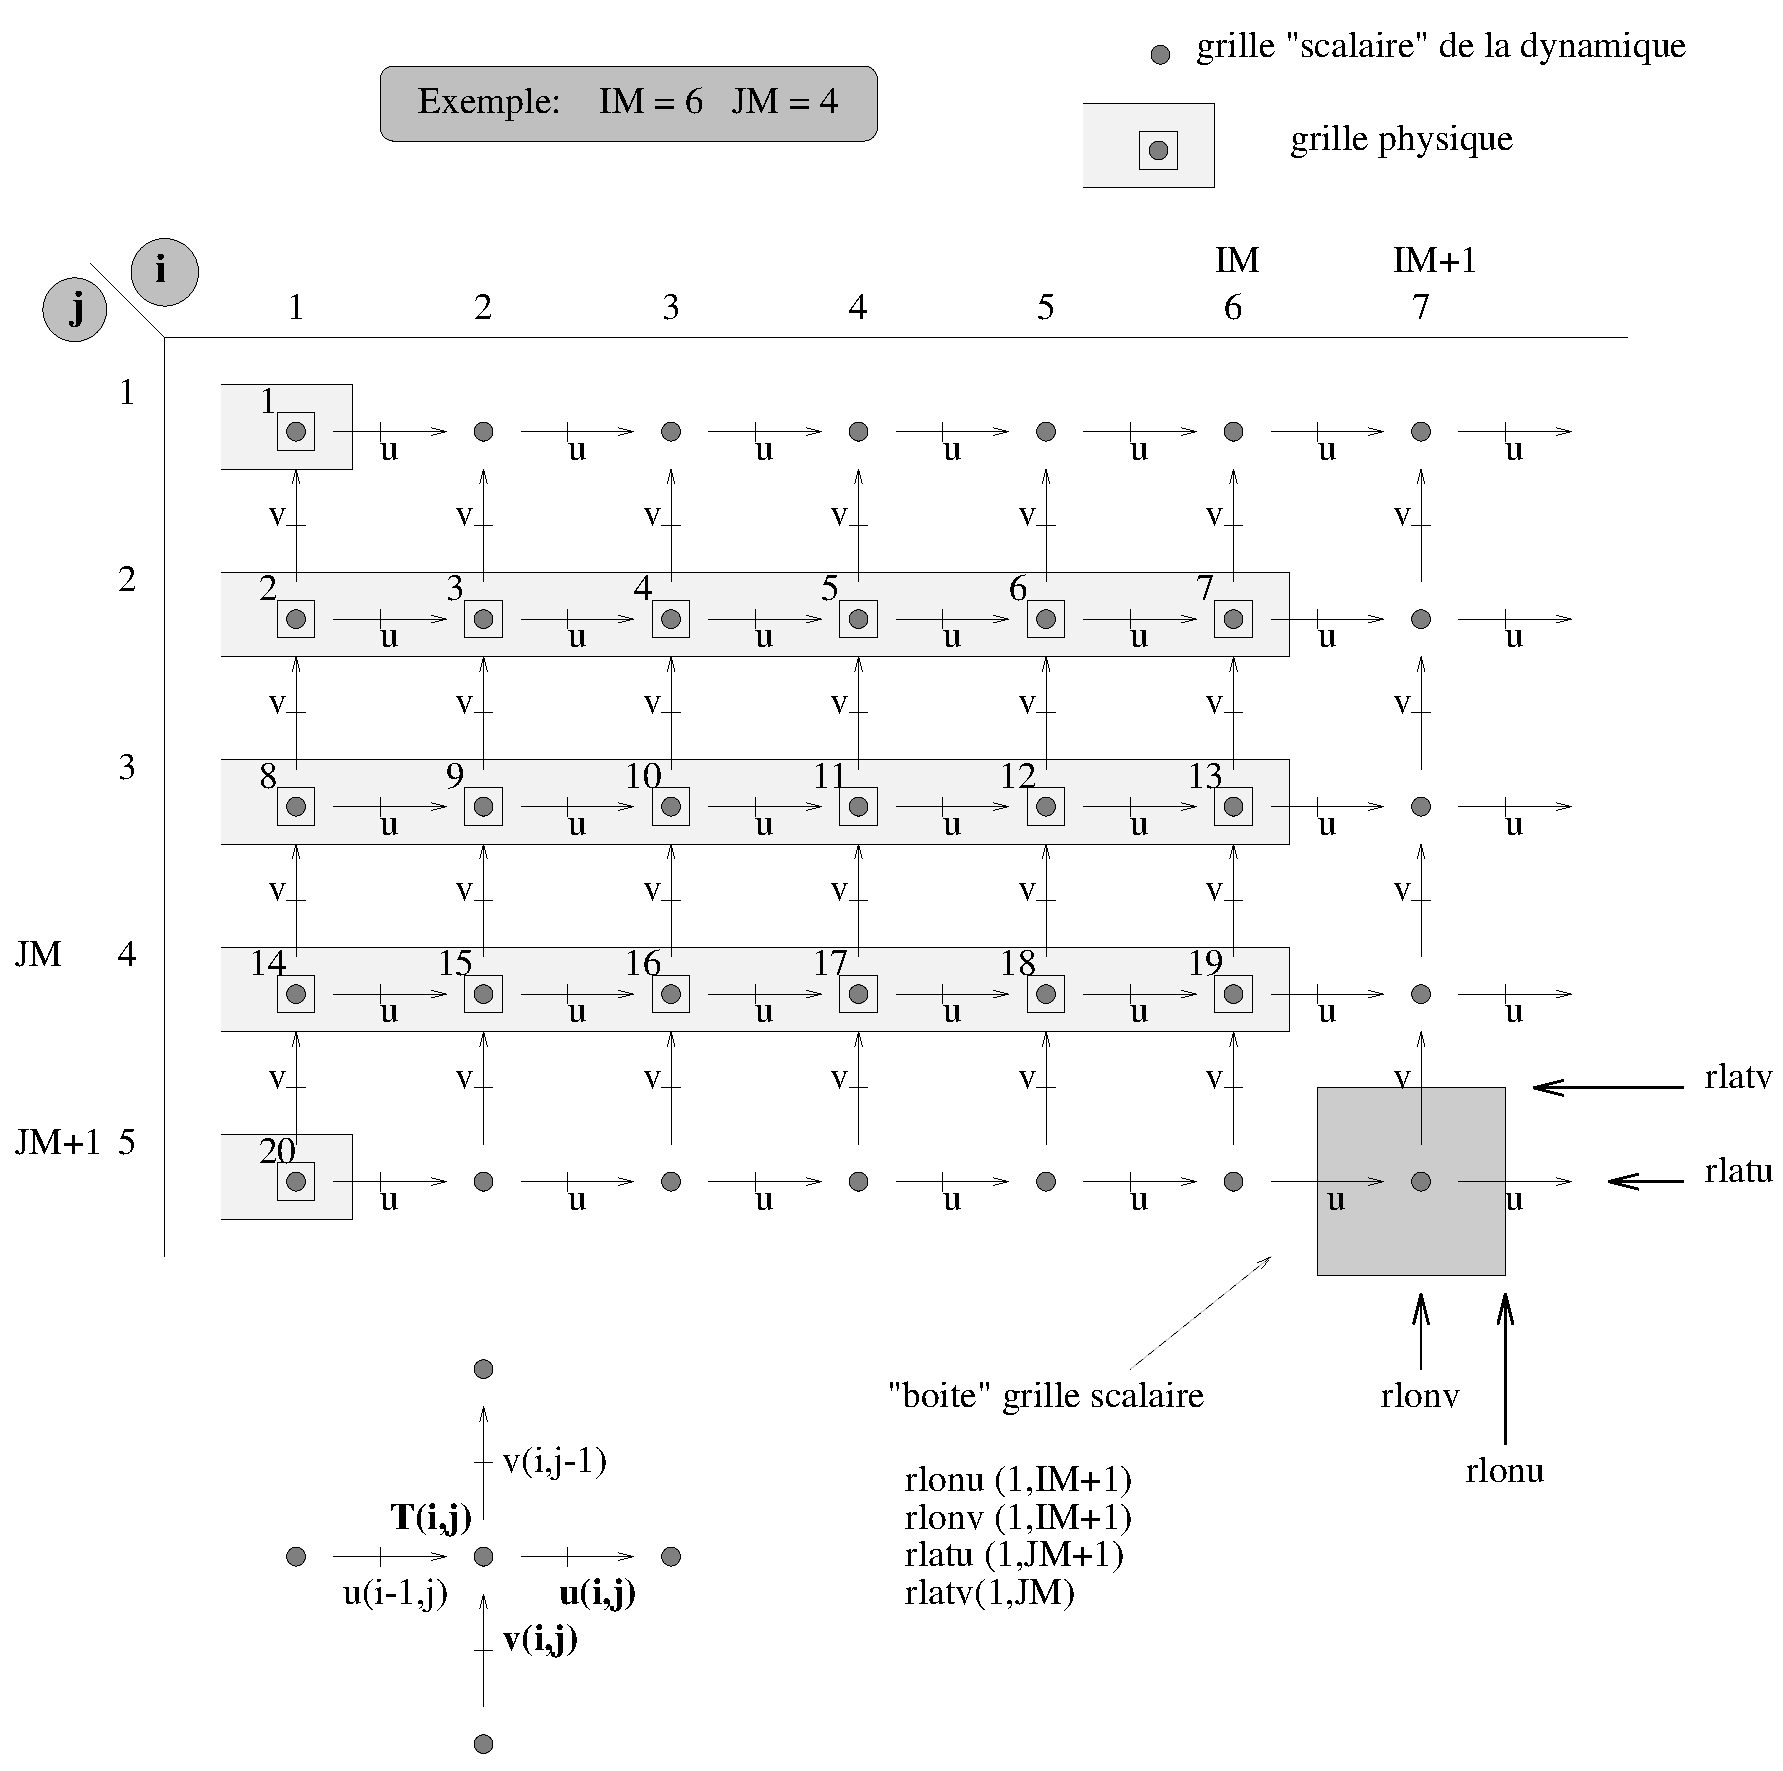
\includegraphics[width=1.2\textwidth]{Fig/grid.eps}}}
\caption{Dynamical and physical grids for a 6 $\times$ 7 horizontal resolution.
In the dynamics (but not in the physics) winds u and v are on specific
staggered grids. Other dynamical variables are on the dynamical ``scalar'' grid.
The physics uses the same ``scalar'' grid for all the variables,
except that nodes are indexed in a single vector containing
NGRID=2+(JM-1)$\times$IM points when counting from the north pole.
N.B.: In the Fortran program, the following variables are used:
 {\tt iim=IM , iip1=IM+1, jjm=JM , jjp1=JM+1}.\label{fg:grid}}
\end{figure}


Dynamics and physics use different grids.
Figure~\ref{fg:grid} shows the correspondence and indexing
of the physical and dynamical grids
as well as the different locations of variables on these grids.
To identify the coordinates of a variable (at one grid point up,
down, right or left)
we use coordinates {\tt rlonu}, {\tt rlatu},
 {\tt rlonv}, {\tt rlatv} (longitudes and
latitudes, in {\bf radians}).

On the dynamical grid, values at {\tt i=1} are the same as at {\tt i=IM+1}
as the latter node is a redundant point (due to the periodicity in longitude,
these two nodes are actualy located at the same place).
Similarly, the extreme {\tt j=1} and {\tt j=JM+1} nodes on the
dynamical grid (respectively corresponding to North and South poles)
are duplicated IM+1 times.\\
In contrast, the physical grid does not contain redundant points
(only one value for each pole and no extra point along longitudes),
as shown in figure~\ref{fg:grid}.
In practice, computations relative to the physics are made
for a series of {\tt ngrid} atmospheric
columns, where {\tt NGRID}={\tt IM}x({\tt JM}-1)+2.

\subsection{Vertical grids}

\begin{figure}[htbp]

{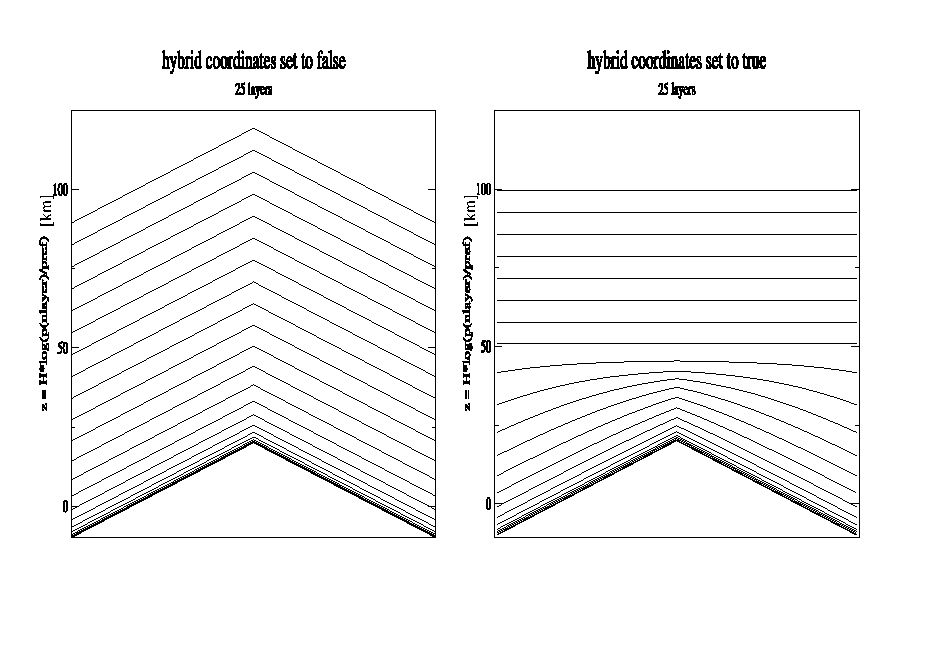
\includegraphics[scale=0.85,clip=true]{Fig/coord.eps}}
\caption[hybrides]
 {Sketch illustrating the difference between hybrid and non-hybrid coordinates}
 \label{fg:hybrid}
\end{figure}


The GCM was initially programmed using sigma coordinates $\sigma = p/ps$
(atmospheric pressure over surface pressure ratio)
which had the advantage of using a constant domain
($\sigma=1$ at the surface and $\sigma=0$ at the top of the atmosphere)
whatever the underlying topography.
However, it is obvious that these coordinates significantly disturb
the stratospheric dynamical representation as the topography is propagated
to the top of the model by the coordinate system.
This problem can elegantly be solved by using a hybrid sigma-P (sigma-pressure)
hybrid coordinate which is equivalent to using $\sigma$ coordinates
near the surface and gradually shifting to purely pressure $p$
coordinates with increasing altitude.
Figure~\ref{fg:hybrid} illustrates the importance of using these
hybrid coordinates compared to simple $\sigma$ coordinates.
The distribution of the vertical layers is irregular,
to enable greater precision at ground level.
In general we use 25 levels to describe the atmosphere to a height of 80 km,
32 levels for simulations up to 120~km, or 50 levels to rise
up to thermosphere.
The first layer describes the first few meters above the ground,
whereas the upper layers span several kilometers.
Figure~\ref{fg:sigma} describes the vertical grid representation
and associated variables.

\begin{figure}
\begin{verbatim}
DYNAMICS                                               PHYSICS
--------                                               -------
[coordinates ap(),bp()]                                [pressures]

ap(llm+1)=0,bp(llm+1)=0  ****************************  plev(nlayer+1)=0
aps(llm),bps(llm)        .. llm .......... nlayer ...  play(nlayer)
ap(llm),bp(llm)          ****************************  plev(nlayer)
aps(llm-1),bps(llm-1)    .. llm-1 ........ nlayer-1 .  play(nlayer-1)
ap(llm-1),bp(llm-1)      ****************************  plev(nlayer-1)
                             :                :
                             :                :
                             :                :
aps(2),bps(2)            ... 2  ............. 2  ....  play(2)
ap(2),bp(2)              ****************************  plev(2)
aps(1),bps(1)            ... 1  ............. 1  ....  play(1)
ap(1)=0,bp(1)=1          **********surface***********  plev(1)=Ps
\end{verbatim}
\caption{Vertical grid description of the {\tt llm (or nlayer)}
atmospheric layers
in the programming code ({\tt llm} is the variable used in the dynamical part,
and {\tt nlayer} is used in the physical part).
Variables {\tt ap, bp} and {\tt aps, bps} indicate the hybrid levels at
the interlayer levels and at middle of the layers respectively.
Pressure at the interlayer is  $Plev(l)=ap(l)+bp(l) \times Ps$ and pressure
in the middle of the layer is defined by $Play(l)=aps(l)+bps(l) \times Ps$,
(where $Ps$ is surface pressure).
Sigma coordinates are merely a specific case of hybrid
coordinates such that $aps=0$ and $bps=P/Ps$.
Note that for the hybrid coordinates, $bps=0$ above $\sim50$~km, leading to
purely pressure levels.
The user can choose whether to run the model using hybrid coordinates or not
by setting variable {\tt hybrid} in run.def to True or False.}
\label{fg:sigma}
\end{figure}

\section{Variables used in the model}

\subsection{Dynamical variables}
The dynamical state variables are the atmospheric temperature,
surface pressure, winds and tracer concentrations.
In practice, the formulation selected to solve the equations in
the dynamics %(see chapter~\ref{sc:dynamic})
is optimised using the following less ``natural'' variables:

\begin{description}
\item - {\bf potential temperature} $\theta$ ({\tt teta} in the code),
linked to temperature {\bf T} by $\theta = T{(P/Pref)}^{-\kappa}$
with $\kappa = R/C_p$
(note that $\kappa$ is called {\tt kappa} in the dynamical code, and {\tt rcp}
in the physical code). We take $Pref=610$ Pa on  Mars.
\item - {\bf surface pressure} ({\tt ps} in the code).
\item - {\bf mass} the atmosphere mass in each grid box ({\tt masse}
in the code).
\item - {\bf the covariant meridional and zonal winds}
{\tt ucov} and {\tt vcov}.
These variables are linked to the "natural" winds by
\verb+ucov = cu * u+ and \verb+vcov = cv * v+, where
\verb+cu+ and \verb+cv+ are constants that only depend on the latitude.
%(see Appendix A).
\item - {\bf mixing ratio of tracers} in the atmosphere, typically
expressed in kg/kg (array {\tt q} in the code).
\end{description}

{\tt ucov} and {\tt vcov}, ``vectorial'' variables, are stored on
``scalari'' grids u and v respectively, in the dynamics
(see section \ref{fg:grid}).
{\tt teta}, {\tt q}, {\tt ps}, {\tt masse}, ``scalar variables'',
are stored on the ``scalar'' grid of the dynamics.



\subsection{Physical variables}

In the physics, the state variables of the dynamics are transmitted
via an interface that interpolates the winds on the scalar grid
(that corresponds to the physical grid) and transforms the dynamical variables
into more ``natural'' variables.
Thus we have winds {\bf u} and  {\bf v} (m.s$^{-1}$),
temperature {\bf T} (K), pressure at the middle of the layers
{\bf play} (Pa) and at interlayers {\bf plev} (Pa), tracers
{\bf q}, etc. (kg/kg) on the same grid.

Furthermore, the physics also handle the evolution of the purely
physical state variables:
\begin{description}
\item - {\bf tsurf} surface temperature (K)
\item - {\bf tsoil} temperature at different layers under the surface (K)
\item - {\bf emis} surface emissivity
\item - {\bf alb} surface albedo
\item - {\bf q2} wind variance, or more precisely the square root of
the turbulent kinetic energy
\item - {\bf qsurf} tracer on the surface (kg.m$^{-2}$)
\item - {\bf rnat} surface type (0 = ocean, 1 = continent)
\item - {\bf beta} surface wetness (0 $\to$ 1 implies dry $\to$ saturated)
\item - [anything else?]
\end{description}

\subsection{Tracers}
The model may include different types of tracers:
\begin{description}
\item - condensed species (e.g., CO$_2$, H$_2$O, dust)
\item - chemically active species (in principle only at the moment)
\item - radiatively active gases (e.g., water vapor)
\end{description}

In the code, all tracers are stored in one three-dimensional array {\tt q},
the third index of which corresponds to each individual tracer.
In input and output files (``start.nc'', ``startfi.nc'',
see Section~\ref{loc:contact1}) tracers are stored separately using their
individual names. Loading specific tracers requires that
the approriate tracer names are set in the {\tt traceur.def} file
(see Section~\ref{sc:traceur.def}), and specific computations
for given tracers (e.g. computing the water or CO$_2$ cycles) 
is controlled by setting the corresponding options in the
{\tt callphys.def} file (see Section~\ref{sc:callphys.def}).


%\chapter{3-D Dynamic code}
\label{sc:dynamic}
{\it\bg  Nul besoin de lire cette partie technique pour travailler avec le GCM!}
\section{Discretisation of the dynamic equations}
\index{The hydrodynamic code}


% definitions pour les formules mathematiques
%\newcommand{\dep}[1]{\left( #1 \right) }
%\newcommand{\depb}[1]{\left[ #1 \right] }
%\newcommand{\depc}[1]{\left\{ #1 \right\} }
\newcommand{\deriv}[1]{\frac{\partial }{\partial #1} }
\def\abs#1{\left| #1 \right|}
\renewcommand{\-}[1]{$^{-#1}$}

% definitions pour la dynamique
\newcommand{\dt}[1]{\frac{\partial #1}{\partial t}}
\newcommand{\dsig}[1]{\deriv{\sigma} \dep{#1} }
\newcommand{\diverg}[1]{\vec{\nabla}.\dep{#1 \vec{V}} }
%\newcommand{\der}[2]{\frac{\partial #1 }{\partial #2} }
\def\ps{p_s}
\def\t{\theta}
\def\w{\dot{\sigma}}
\def\cp{C_p}
\def\rcp{\kappa}

%
%   ATTENTION  ne plait pas a latex2html (I don't know why)
%       de toutes facons inutile
%\def\p0{p_0}
%\def\s{ {\dep{\frac{p}{\p0}}}^{\rcp} }
%

\newcommand{\adv}[1]{\diverg{\ps #1} + \dsig{\ps #1 \dot{\sigma}} }

\def\sc#1{Section~\ref{sc:#1}}
\def\an#1{Annexe~\ref{an:#1}}
\def\ch#1{Chapitre~\ref{ch:#1}}
\def\fig#1{Fig.~\ref{fg:#1}}
\def\figs#1{Figs.~\ref{fg:#1}}
\def\eq#1{Eq.~\ref{eq:#1}}
\def\eqs#1{Eqs.~\ref{eq:#1}}
\def\tb#1{Table~\ref{tb:#1}}
%\newcommand{\av}[2]{{\overline{#1}}^{ #2 }}
%\newcommand{\avg}[1]{\left< #1 \right>}
\def\cd{C_D}
\def\dx{\delta_X}
\def\dy{\delta_Y}
\def\dz{\delta_Z}

\def\filtre{{\cal F}}
\def\uabs{\tilde{u}_{a}}
\def\err{\epsilon}
\def\dsig{\dz \sigma}
\def\psk{{\ps}^\kappa}
\def\ucov{\tilde{u}}
\def\vcov{\tilde{v}}
\def\ucont{\tilde{\ucov}}
\def\vcont{\tilde{\vcov}}
\def\cu{c_u}
\def\cv{c_v}
\def\h{\theta}
\def\pext{\tilde{p}_s}
\def\fext{f}
\def\K{\frac{1}{2}
\left( \av{\ucov \ucont}{X} + \av{\vcov \vcont}{Y} \right)}
\def\Z{\frac{\filtre\dep{\dx \vcov - \dy \ucov} + \fext}{\av{\pext}{X,Y}}}
\def\Zm{\frac{- \dy \ucov + \fext}{\av{\pext}{Y}}}

\newcommand{\glob}[1]{ \left< #1 \right> }

%\centerline{Robert Sadourny, Phu Le Van, Fr\'ed\'eric Hourdin}
%\centerline{Laboratoire de M\protect\'et\protect{\'e}orologie Dynamique du CNRS}
%\centerline{Ecole Normale Sup\protect{\'e}rieure}
%\centerline{24 rue Lhomond}
%\centerline{75231 PARIS cedex 05}
%\centerline{FRANCE}
%\vspace{1cm}

%\begin{center}
%Robert Sadourny, Phu Le Van, Fr\'ed\'eric Hourdin\\
%Laboratoire de M\protect\'et\protect{\'e}orologie Dynamique du CNRS\\
%Ecole Normale Sup\protect{\'e}rieure\\
%24 rue Lhomond\\
%75231 PARIS cedex 05\\
%FRANCE
%\end{center}

{\it Extrait de la note de Robert Sadourny, Phu Le Van et Fr\'ed\'eric
Hourdin, Laboratoire de M\protect\'et\protect{\'e}orologie Dynamique}.\\


Le mod\`ele climatique du LMD est b\^ati, comme tous les
mod\`eles de circulation g\'en\'erale atmosph\'erique,
sur la r\'esolution num\'erique des {\'equations primitives
de la m\'et\'eorologie} d\'ecrites dans de nombreux
ouvrages~\cite{Holt:79}.
L'analyse pr\'esent\'ee ici a \'et\'e men\'ee sur la nouvelle
version de la dynamique du LMD \'ecrite par Phu Le Van~\cite{LeVa:89}
sur une formulation de Robert Sadourny.
Cette formulation diff\`ere de l'ancienne essentiellement
par deux points:
dans la nouvelle formulation, la r\'epartition des points en
longitude et en latitude peut \^etre chang\'ee arbitrairement.
L'autre modification porte sur la r\'epartition des points
aux p\^oles\footnote{Aux p\^oles sont calcul\'es:
le vent m\'eridien dans l'ancienne formulation et les variables
scalaires dans la nouvelle.}.

La coordonn\'ee  verticale du mod\`ele est la pression normalis\'ee
par sa valeur \`a la surface: $\sigma=p/\ps$.
On utilise en fait $\sigma$ aux niveaux inter-couches
et $s=\sigma^\kappa$ au milieu des couches.
On note $X$ et $Y$ les coordonn\'ees horizontales:

\begin{figure}
\begin{center}
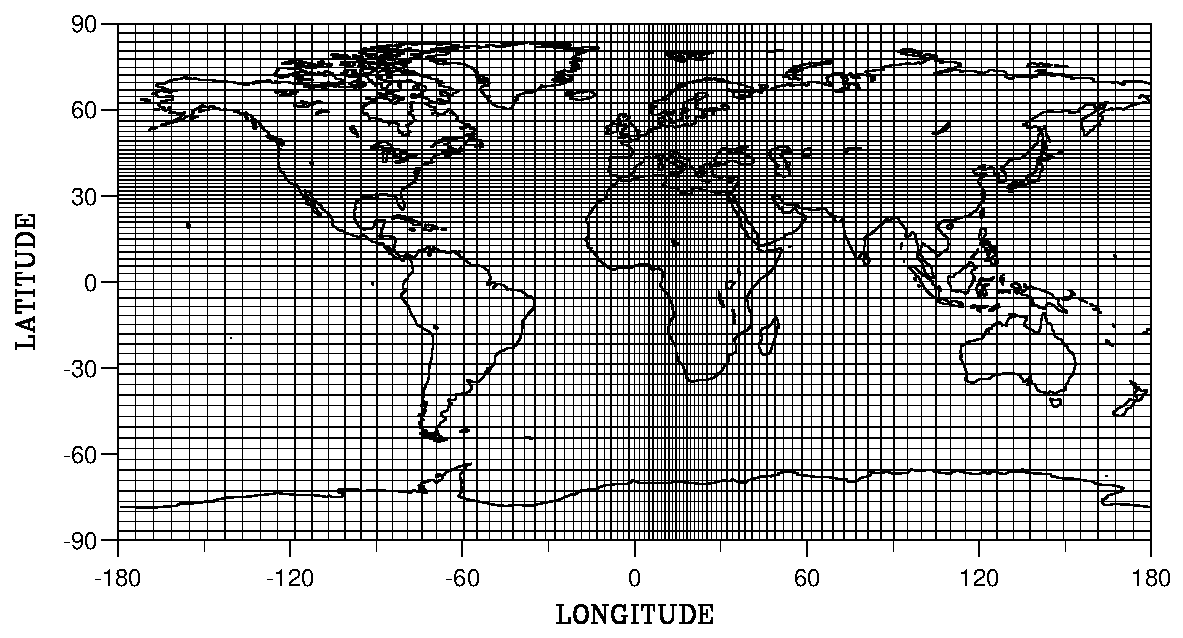
\includegraphics[width=13cm]{Fig/glob.eps}
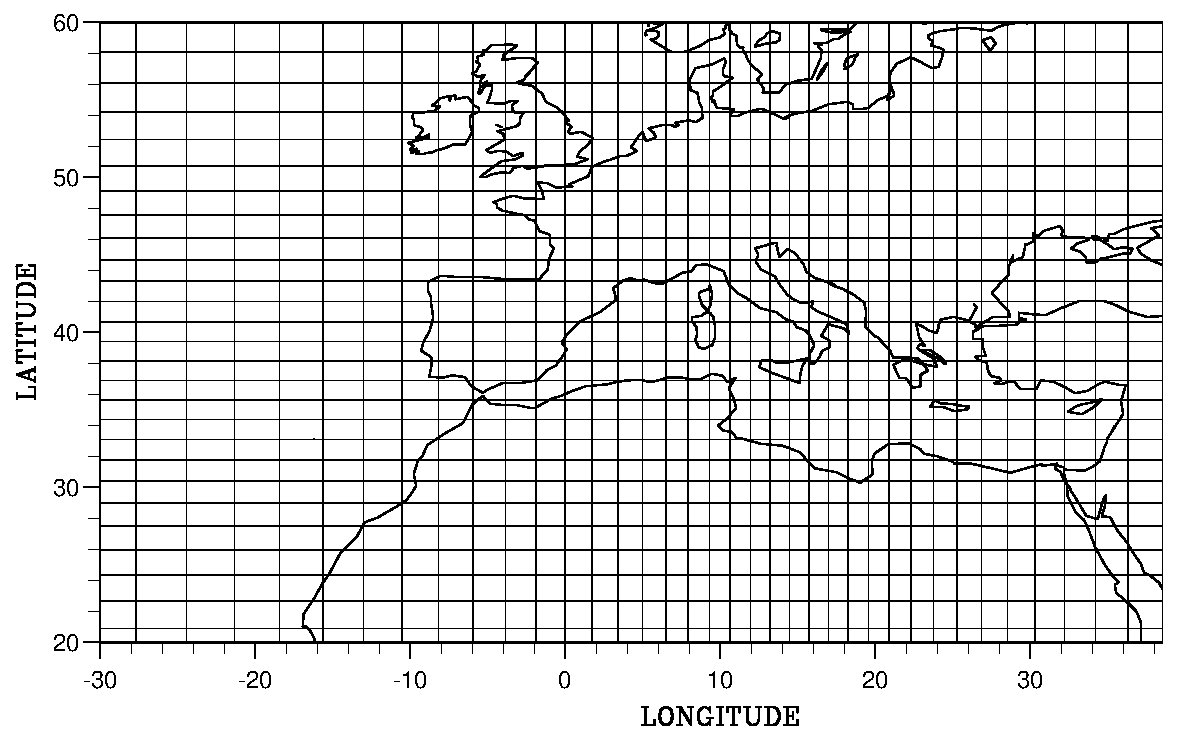
\includegraphics[width=10cm]{Fig/med.eps}
\caption{Grille obtenue avec 96 points en longitude et 73 en latitude et
un zoom d'un facteur 3 centr\'e sur la m\'edit\'erann\'ee (grille utilis\'ee au laboratoire par Ali Harzallah)\label{fg:zoom}}.
\end{center}
\end{figure}

$X$ (resp. $Y$) est une fonction biunivoque de la longitude $\lambda$
(resp. de la latitude $\phi$). Ces deux fonctions peuvent \^etre choisies
de fa\c{c}on arbitraire dans le mod\`ele LMDZ ce qui permet d'effectuer un
zoom sur une r\'egion du globe particuli\`ere. Une grille de ce type est montr\'ee
sur la Figure~\ref{fg:zoom}.
Les variables scalaires
(temp\'erature potentielle $\h = c_p T/\psk$, g\'eopotentiel $\Phi$
et pression de surface $\ps$) sont \'evalu\'ees aux points
correspondant \`a des couples de valeurs enti\`eres $(X,Y)=(i,j)$.
Les variables dynamiques sont d\'ecal\'ees par rapport aux variables
scalaires en utilisant une grille $C$ dans la d\'efinition de
Arakawa~\cite{Arak:77}: le vent zonal est calcul\'e
aux points $(X,Y)=(i+1/2,j)$ et  le vent
m\'eridien aux points $(X,Y)=(i,j+1/2)$.
La disposition des variables sur la grille est illustr\'ee sur la
Figure~\ref{fg:grille}.

\begin{figure}
\centerline{\framebox{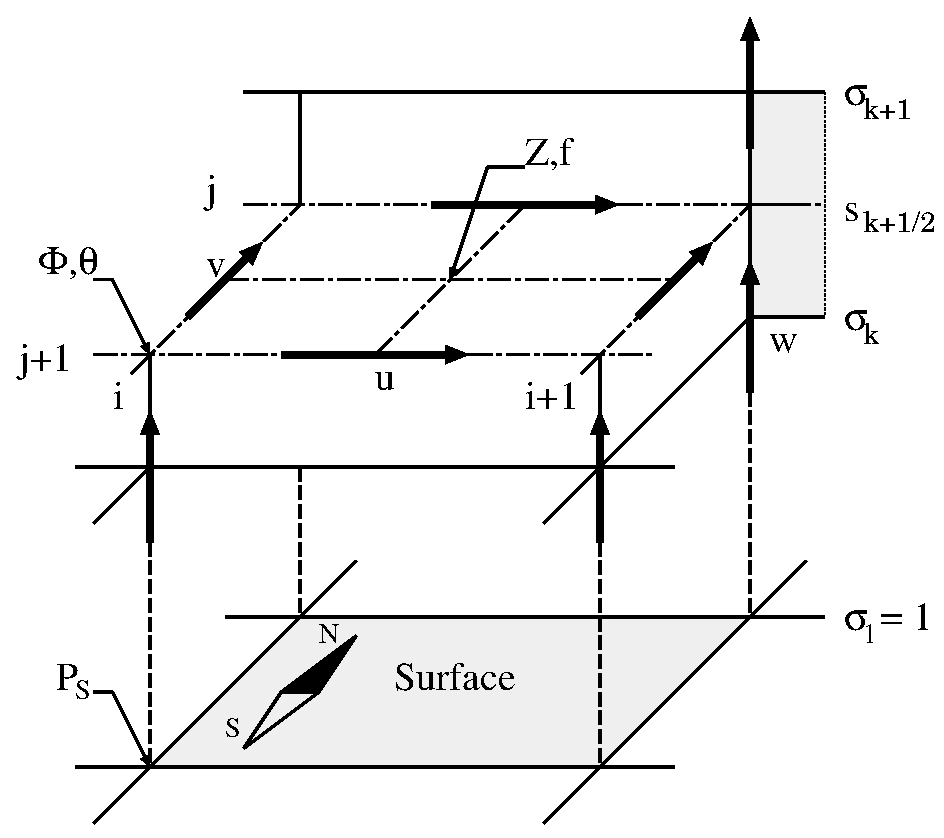
\includegraphics[width=0.6\textwidth]{Fig/grille.eps}}}
\caption{Disposition des variables dans la grille du LMD}
\label{fg:grille}
\end{figure}


On utilise en fait les composantes covariantes
($\ucov$ et $\vcov$) et contravariantes ($\ucont$ et $\vcont$)
du vent d\'efinies par
\begin{equation}
\begin{array}{llllllllll}
\ucov = \cu u & \mbox{et} & \ucont = u / \cu & \mbox{avec} & 
\cu = a \cos{\phi} \left( d\lambda/dX \right)  \\
\vcov = \cv v & \mbox{et} & \vcont = v / \cv & \mbox{avec} &
\cv = a \left( d\phi / dY \right)
\end{array}
\end{equation}
%
o\`u $u$ et $v$ sont les composantes physiques du vecteur vent
horizontal.
On introduit \'egalement:
%
\paragraph{la pression extensive:}
$\pext$ (pression au sol multipli\'ee
par l'aire de la maille).
%
\paragraph{les trois composantes du flux de masse:}
\begin{equation}
U=\av{\pext}{X} \ucont ,\  V= \av{\pext}{Y} \vcont \  \mbox{et} \  
W= \pext \dot{\sigma}
\ \mbox{avec}\ \dot{\sigma}=\frac{d\sigma}{dt}
\end{equation}
%
\paragraph{le facteur de Coriolis multipli\'e par l'aire de la maille:}
$\fext=2\Omega \sin{\phi} \cu \cv$\\
o\`u $\Omega$ est la vitesse de rotation de la plan\`ete.
%
\paragraph{la vorticit\'e potentielle absolue:}
\begin{equation}
Z=\Z
\end{equation}
%
\paragraph{l'\'energie cin\'etique}
\begin{equation}
K=\K
\end{equation}\\
%
La notation $\delta X$ signifie simplement qu'on
effectue la diff\'erence entre deux points cons\'ecutifs
suivant la direction $X$.
La notation $\av{a}{X}$ signifie qu'on prend la moyenne arithm\'etique
de la quantit\'e $a$ suivant la direction $X$. $\filtre$ est un filtre longitudinale appliqu\'e dans les r\'egions polaires.
Les \'equations discr\'etis\'ees sont \'ecrites sous la forme
suivante:
\paragraph{\'equations du mouvement:}
\begin{equation} \label{eq:u1}
\dt{\ucov} -
\av{Z}{Y} \av{V}{X,Y} 
+ \dx \filtre\dep{\Phi + K}
+s \av{\h}{X} \dx \filtre\dep{\psk}
- \frac{\av{\uabs}{Y,Y} \dz \av{W}{X} }
{\av{\pext}{X} \dsig }
+ \frac{\dz \left( \av{W}{X} \av{\uabs}{Z} \right) }
{\av{\pext}{X} \dsig}
=S_{\ucov}
\end{equation}
o\'u $\uabs$ est la composante zonale covariante
du vecteur vent absolu:
$\uabs=\ucov+\cu a \Omega \cos{\phi}$ et
\begin{equation} \label{eq:v1}
\dt{\vcov} + \av{Z}{X} \av{U}{X,Y} + \dy \filtre\dep{\Phi + K}
+s \av{\h}{Y} \dy \filtre\dep{\psk}
- \frac{\av{\vcov}{X,X} \dz \av{W}{Y} }
{\av{\pext}{Y} \dsig}
+ \frac{\dz \left( \av{W}{Y} \av{\vcov}{Z} \right) }
{\av{\pext}{X} \dsig}
=S_{\vcov}
\end{equation}
%
\paragraph{\'equation thermodynamique:}
%
\begin{equation}
\label{eq:thermo}
\dt{\dep{\pext \h}}
+\filtre\depb{\dx \dep{\av{\h}{X}U} +\dy \dep{\av{\h}{Y}V} }
+\frac{\dz \dep{\av{\h}{Z} W}}{\dz \sigma}=S_\h
\end{equation}
%
\paragraph{\'equation hydrostatique:}
\begin{equation}
\dz \Phi=-\ps^\rcp  \av{\h}{z} \dz s
\end{equation}
%
\paragraph{\'equations de continuit\'e:}
%
\begin{equation}
\label{eq:cont1}
\dt{\ps}  = \filtre\depb{\sum_z{\dz \sigma \dep{\dx U+ \dy V}}}
\end{equation}
\begin{equation}
\label{eq:cont2}
\dz W   = -\dz \sigma \depb{\filtre\dep{\dx U+ \dy V} + \dt{\ps}}
\end{equation}
%
On a not\'e $S$ les termes sources dans les diff\'erentes \'equations.
Dans ces termes sources, on distingue 1) d'une part les param\'etrisations physiques mentionn\'ees plus haut et qui font intervenir pour une maille donn\'ee du mod\`ele, tous les points situ\'es sur une m\^eme verticale mais ceux-l\`a seulement; 2) les op\'erateurs de dissipation horizontale, cens\'es rendre compte des \'echanges entre \'echelles explicitement repr\'esent\'ees dans le mod\`ele et \'echelles sous-mailles. Ces op\'erateurs ont la structure de Laplaciens agissant sur des plans horizontaux c'est \`a dire qu'il font intervenir un voisin de chaque c\^ot\'e dans les deux directions horizontales. Cet op\'erateur est g\'en\'eralement it\'er\'e pour le rendre plus s\'electif en \'echelle (plus on it\`ere un laplacien et plus son effet sur les petites \'echelles devient important relativement).

\section{High latitude filters}

{\it Extract adapted from Forget et al. [1999]}\\

At high latitude a filter is applied near
the singularity in the grid at the pole
in order to satisfy the Courant-Friedrichs-Lewy numerical
stability criterion without going to an excessively
small timestep. In the original version of the dynamical code
a classical Fourier filter was used,  but
we found that because the Martian polar
atmosphere appears to be much more dynamically unstable than the Earth's
polar atmosphere, a more efficient formulation (based on the
grouping of adjacent gridpoints together)  was necessary
to avoid numerical instability. \\

{\it In practice the following technique is used in the subroutine called {\em groupeun.F} :
\begin{itemize}
\item The points are grouped in packets of $2^{\mbox{ngroup}}$
      at the poles(e.g. {\bf ngroup}=3 $\rightarrow$ packets of 8),
 then $2^{\mbox{ngroup-1}}$,
      $2^{\mbox{ngroup-2}}$, etc. in the lower latitudes moving away from the pole
 
   \item The higher {\bf ngroup} is, the more efficient the smoothing is, and the more stable the model.
 
\item   BUT, {\bf iim} must be divisible by $2^{\mbox{ngroup}}$ !!!
 

\end{itemize}

}


\section{Dissipation}

{\it Extract adapted from Forget et al. [1999]}\\

In the LMD grid point model,
nonlinear interactions between explicitly resolved scales
and subgrid-scale processes are
parameterized by applying a scale-selective horizontal
dissipation operator
based on an $n$ time iterated Laplacian $\Delta^{n}$.
For the grid point model, for instance, this can be written
${\partial q}/{\partial t} = ([-1]^{n}/ {\tau_{\mbox{\scriptsize
diss}}})
(\delta x)^{2n} \Delta^{n} q$
where $\delta x$ is the smallest horizontal distance represented in the
model and $\tau_{\mbox{\scriptsize diss}}$ is the dissipation timescale
for a st
ructure of scale
$\delta x$.
These operators are necessary to ensure the grid point model
numerical stability.
In practice, the operator is
separately applied to (1)~potential temperature, (2)~the divergence of
the flow,
and (3)~its vorticity.
We respectively use  $n=2$, $n=1$, and $n=2$ in the grid point model.\\

{\it Note: In practice,
values of $n$ and $\tau_{\mbox{\scriptsize diss}}$
are adjustable and prescribed at the beginning of each run, in run definition file ``run.def'' (cf.~\ref{vb:run.def}) } 

\section{Sponge layer}

{\it Extract adapted from Forget et al. [1999]}\\

In the upper levels a sponge layer is also used in both models
in an attempt to reduce
spurious reflections of vertically propagating waves from the model top.
Unlike the traditional Rayleigh friction formulation,
this operates as a linear drag
 solely on the eddy components of the vorticity and divergence
fields and is not scale-selective.  The timescales on which it operates
are
typically half a day, 1 day,  and 2 days
 at the three uppermost levels, respectively. \\

{\it Note: the sponge layer ``timescale'' values and their extensions in altitude
are adjustable and prescribed at the beginning of each run, in run definition file ``run.def'' (cf.~\ref{vb:run.def}) } 








\chapter{The physical parameterizations of the Martian model: some references}

\label{sc:phymars}

\section{General}

The Martian General Circulation Model uses a large number of physical
parameterizations based on various scientific theories
and some generated using specific numerical methods.

A list of these parameterizations is given below, along with the most
appropriate
references for each one. Most of these documents can be consulted at:
\verb+http://www-mars.lmd.jussieu.fr/mars/publi.html+.


\paragraph{General references:}
A document attempts to give a complete scientific description of the current
version of the GCM (a version without tracers): 
\begin{itemize}
\item  {\it Forget et al.} [1999] (article
published in JGR) 
\end{itemize}

\nocite{Forg:99}

\section{Radiative transfer}

The radiative transfer parameterizations are used to calculate the heating
and cooling ratios in the atmosphere and the radiative flux at the surface.

\subsection{\bf CO$_2$ gas absorption/emission:}
\subsubsection*{Thermal IR radiation} (\verb+ lwmain+)
\begin{itemize}
\item New numerical method, solution for the radiative transfer equation:
{\it Dufresne et al.} [2005]. 
\item Model validation and inclusion of the ``Doppler'' effect
(but using an old numerical formulation):
{\it Hourdin} [1992] (article).
\nocite{Hour:92,Hour:00b,Dufr:05}

\item At high altitudes, parameterization of the thermal radiative transfer
({\tt nltecool}) when the local thermodynamic balance is no longer valid
(e.g. within 0.1 Pa) : Lopez-Valverde et al. [2001] :
Report for the ESA available on the web
as: ``CO2 non-LTE cooling rate at
15-um and its parameterization for the Mars atmosphere''.

\end{itemize}

\subsubsection*{Absorption of near-infrared radiation}
 (\verb+ nirco2abs+)
\begin{itemize}
\item {\it Forget et al.} [1999]
\end{itemize}

\subsection{\bf Absorption/emission and diffusion by dust:}

\subsubsection*{Dust spatial distribution}
 (\verb+ aeropacity+)

\begin{itemize}
\item The method for semi-interactive dust vertical distribution
is detailed in {\it Madeleine et al.} [2011]
\item Vertical distribution and description of ``MGS'' and ``Viking'' scenarios
in the ESA report {\it Mars Climate Database V3.0 Detailed Design Document}
by Lewis et al. (2001), available on the web.
\item For the ``MY24''-``MY26'' scenarios, the dust distributions were
derived from observations made by
TES data is used. See technical note WP12.2.1 of ESA contract
Ref~ESA 11369/95/NL/JG(SC) "New dust scenarios for the Mars Climate Model : Martian Years
24-29", available online at
\verb+http://www-mars.lmd.jussieu.fr/WP2011/wp12.1.1.pdf+

\end{itemize}
\nocite{Lewi:99,Made:11}

\subsubsection*{Thermal IR radiation}
 (\verb+ lwmain+)
\begin{itemize}
\item Numerical method:  {\it Toon et al.} [1989] 
\item Optical properties of dust:  {\it Madeleine et al.} [2011] 
\nocite{Toon:89,Made:11}
\end{itemize}

\subsubsection*{Solar radiation}
 (\verb+ swmain+)
\begin{itemize}
\item Numerical method: {\it Toon et al.} [1989]
\nocite{Toon:89}

\item Optical properties of dust: 
see the discussion in {\it Madeleine et al.} [2011], which quotes
properties from {\it Wolff et al.} [2009].
\nocite{Made:11,Wolf:09}
\end{itemize}

\section{Subgrid atmospheric dynamical processes}

\subsection{Turbulent diffusion in the upper layer}
 (\verb+ vdifc+)

\begin{itemize}
\item Implicit numerical scheme in the vertical:
see the thesis of Laurent Li (LMD, Universit\'e Paris 7, 1990), Appendix C2.

\item Calculation of the turbulent diffusion coefficients:
{\it Forget et al. } [1999].

\item fluxes in the near-surface layer: {\it Colaitis et al.} [2012],
technical note WP13.1.3d of ESA contract
Ref~ESA 11369/95/NL/JG(SC) "New Mars Climate Model:
d) New convection and boundary layer schemes and their impact on
Mars meteorology", available online at 
\verb+http://www-mars.lmd.jussieu.fr/WP2011/wp13.1.3d.pdf+

\end{itemize}

\subsection{Convection}
 (\verb+ convadj+)
\begin{itemize}
\item For some details on the convective adjustement,
see {\it Hourdin et al.} [1993]
\item The thermals' mass flux scheme is described in
{\it Colaitis et al.} [2012],
technical note WP13.1.3d of ESA contract
Ref~ESA 11369/95/NL/JG(SC) "New Mars Climate Model:
d) New convection and boundary layer schemes and their impact on
Mars meteorology", available online at 
\verb+http://www-mars.lmd.jussieu.fr/WP2011/wp13.1.3d.pdf+
\end{itemize}
\nocite{Hour:93}
 
\subsection{Effects of subgrid orography and gravity waves}
 (\verb+ calldrag_noro+ ,  \verb+ drag_noro+ )

See {\it Forget et al. } [1999] and {\it Lott and Miller} [1997]
\nocite{Lott:97}

\section{Surface thermal conduction}
 (\verb+soil+)

The numerical scheme is described in section 2 of technical note
WP11.1 of ESA contract
Ref~ESA 11369/95/NL/JG(SC) "Improvement of the high latitude
processes in the Mars Global Climate Model", available online at
\verb+http://www-mars.lmd.jussieu.fr/WP2008/Polar_processes.pdf+
 
\section{CO$_2$ Condensation}

\begin{itemize}
\item In {\it Forget et al.} [1998] (article published in Icarus):
 \begin{itemize}
  \item Numerical method for calculating the condensation and sublimation levels
at the surface and in the atmosphere (\verb+ newcondens+)
 explained in the appendix.
  \item Description of the numerical scheme for calculating the evolution of CO$_2$
snow emissivity (\verb+co2snow+) explained in section 4.1
  \end{itemize}
\nocite{Forg:98}
\item Noncondensable gaz treatment: see {\it Forget et al.} [2008],
available online at
\verb+http://www.lpi.usra.edu/meetings/modeling2008/pdf/9106.pdf+
\item Inclusion of sub-surface water ice table thermal effect, varying albedo
of polar caps and tuning of the CO2 cycle are descibed in technical note
WP13.1.3e of ESA contract
Ref~ESA 11369/95/NL/JG(SC) "New Mars Global Climate Model:
e) Improved CO2 cycle and seasonal pressure variations", available online at
\verb+http://www-mars.lmd.jussieu.fr/WP2011/wp13.1.3e.pdf+
\end{itemize}


\section{Tracer transport and sources} 
\begin{itemize}
\item ``Van-Leer'' transport scheme used in the dynamical part
(\verb+ tracvl+ and  \verb+ vlsplt+ in the dynamical part):
{\it Hourdin and Armengaud} [1999] \nocite{Hour:99}

\item Transport by turbulent diffusion  (in \verb+ vdifc+), convection
(in  \verb+ convadj+), sedimentation  (\verb+ sedim+),
dust lifting by winds (\verb+ dustlift+) :
see note ``Preliminary design of dust lifting and transport in the Model''
(ESA contract, Work Package 4, 1998, available on the web). 

\item Dust transport by the ``Mass mixing ratio /
Number mixing ratio'' method for grain size evolution: see article by {\it
Madeleine et al.} [2011]
\nocite{Made:11}

%\item Simplified water cycle (source in {\tt vdifc}, {\tt
%watercloud}) : and also see the Maitrise study by Delphine Nobileau, LMD, 2000.
\item {\bf Watercycle}, see {\it Montmessin et al.} [2004]
and technical note
WP13.1.3c of ESA contract
Ref~ESA 11369/95/NL/JG(SC) "New Mars Climate Model: c) Inclusion of cloud
microphysics, dust scavenging and improvement of the water cycle",
available online at
\verb+http://www-mars.lmd.jussieu.fr/WP2011/wp13.1.3c.pdf+
\nocite{Mont:04jgr}

\item Radiative effect of clouds: see technical note
WP13.1.3b of ESA contract Ref~ESA 11369/95/NL/JG(SC)
"New Mars Climate Model: b) Radiative effects of water
ice clouds and impact on temperatures", available online at
\verb+http://www-mars.lmd.jussieu.fr/WP2011/wp13.1.3b.pdf+

%\item Chemistry, thermosphere, clouds: currently being published.
\item {\bf Chemistry}, see {\it Lef\`evre et al.} [2004]
and {\it Lef\`evre et al. [2008]}
\nocite{Lefe:04,Lefe:08}
\end{itemize}

\section{Thermosphere}
\begin{itemize}
\item A general description of the model is given in
{\it Gonz{\'a}lez-Galindo et al.} [2009]
\item Details on photochemistry and EUV radiative transfer can be found in
{\it Angelats i Coll et al.} [2005] and
{\it Gonz{\'a}lez-Galindo et al.} [2005]
\end{itemize}
\nocite{Gonz:09a,Gonz:09b,Gonz:05,Ange:05}

{\footnotesize
\begin{verbatim}

#------------------------------
# Parametres de controle du run
#------------------------------

# Nombre de jours d'integration
     nday=669

# nombre de pas par jour (multiple de iperiod) ( ici pour  dt = 1 min )
 day_step = 960

# periode pour le pas Matsuno (en pas)
  iperiod=5

# periode de sortie des variables de controle (en pas)
  iconser=120

# periode d'ecriture du fichier histoire (en jour)
    iecri=100

# periode de stockage fichier histmoy (en jour)
 periodav=60.

# periode de la dissipation (en pas)
  idissip=5

# choix de l'operateur de dissipation (star ou  non star )
 lstardis=.true.

# avec ou sans coordonnee hybrides
 hybrid=.true.

# nombre d'iterations de l'operateur de dissipation   gradiv
nitergdiv=1

# nombre d'iterations de l'operateur de dissipation  nxgradrot
nitergrot=2

# nombre d'iterations de l'operateur de dissipation  divgrad
   niterh=2

# temps de dissipation des plus petites long.d ondes pour u,v (gradiv)
 tetagdiv=10000.

# temps de dissipation des plus petites long.d ondes pour u,v(nxgradrot)
 tetagrot=10000.

# temps de dissipation des plus petites long.d ondes pour  h ( divgrad)
 tetatemp=10000.

# coefficient pour gamdissip
  coefdis=0.

# choix du shema d'integration temporelle (Matsuno ou Matsuno-leapfrog)
  purmats=.false.

# avec ou sans physique
   physic=.true.

# periode de la physique (en pas)
  iphysiq=20

# choix d'une grille reguliere
  grireg=.true.

# frequence (en pas) de l'ecriture du fichier diagfi
 ecritphy=1920

# longitude en degres du centre du zoom
   clon=63.

# latitude en degres du centre du zoom
   clat=0.

# facteur de grossissement du zoom,selon longitude
  grossismx=1.

# facteur de grossissement du zoom ,selon latitude
 grossismy=1.

#  Fonction  f(y)  hyperbolique  si = .true.  , sinon  sinusoidale
  fxyhypb=.false.

# extension en longitude  de la zone du zoom  ( fraction de la zone totale)
   dzoomx= 0.

# extension en latitude de la zone  du zoom  ( fraction de la zone totale)
   dzoomy=0.

#  raideur du zoom en  X
    taux=2.

#  raideur du zoom en  Y
    tauy=2.

#  Fonction  f(y) avec y = Sin(latit.) si = .TRUE. ,  Sinon  y = latit.
  ysinus= .false.

# Avec sponge layer
  callsponge  = .true.

# Sponge:  mode0(u=v=0), mode1(u=umoy,v=0), mode2(u=umoy,v=vmoy)
  mode_sponge= 2

# Sponge:  hauteur de sponge (km)
  hsponge= 90

# Sponge:  tetasponge (secondes)
  tetasponge = 50000

# some definitions for the physics, in file 'callphys.def'
INCLUDEDEF=callphys.def


\end{verbatim}
}

\chapter{Program organization and compilation script}
\label{sc:info}
\index{Programming organization and compilation}

\label{loc:contenu}

All the elements of the LMD model are in the {\bf LMDZ.GENERIC} directory
(and subdirectories).
As explained in Section~\ref{loc:contact1}, this directory
should be associated with
 environment variable {\bf LMDGCM}:\\
If using Csh:
\begin{verbatim}
setenv  LMDGCM /where/you/put/the/model/LMDZ.GENERIC
\end{verbatim}
If using Bash:
\begin{verbatim}
export  LMDGCM=/where/you/put/the/model/LMDZ.GENERIC
\end{verbatim}

\noindent Here is a brief description of the
{\bf LMDZ.GENERIC} directory contents:
\begin{verbatim}
  libf/  All the model FORTRAN Sources (.F or .F90)
         and  include files (.h) organised in sub-directories
        (physics (phystd), dynamics (dyn3d), filters (filtrez)...)

  deftank/   A collection of examples of parameter files required
                to run the GCM (run.def, callphys.def, ...)

  makegcm  Script that should be used to compile the GCM as well
            as related utilities (newstart, start2archive, testphys1d)

  create_make_gcm   Executable used to create the makefile.
                    This command is run automatically by
                    "makegcm" (see below).

\end{verbatim}


\section{Organization of the model source files}
\index{Organization of the model source files}

The model source files are stored in various sub directories
in directory {\bf libf}.
These sub-directories correspond to the different parts of the model:

\begin{description}
\item{\bf grid:} mainly made up of "dimensions.h" file,
which contains the parameters that define the model grid,
i.e. the number of points in longitude (IIM), latitude (JJM) and altitude
(LLM), as well as the number of tracers (NQMX).

\item{\bf dyn3d:} contains the dynamical subroutines.

\item{\bf bibio:} contains some generic subroutines not specifically
related to physics or dynamics but used by either or both.

\item{\bf phymars:} contains the physics routines.

\item{\bf filtrez:} contains the longitudinal filter sources applied in the
upper latitudes,
where the Courant-Friedrich-Levy stability criterion is violated.

\end{description}

\section{Programming}

The model is written in {\bf Fortran-77} and {\bf Fortran-90}.
\begin{itemize}
\item The program sources are written in {\bf ``file.F"}
or {\bf ``file.F90''} files.
The extension .F is the standard extension for fixed-form Fortran and
the extension .F90 is for free-form Fortran.
These files must be preprocessed (by a{\bf C preprocessor}
such as (cpp)) before compilation (this behaviour is, for most
compilers, implicitly obtained but using a capital F in the extention
of the file names).

\item Constants are placed in COMMON declarations,
located in the common ``include'' files {\bf "file.h"}

%\item [also module files now too...]
\item In general, variables are passed from subroutine to subroutine
as arguments (and never as COMMON blocks).

\item In some parts of the code, for ``historical'' reasons,
the following rule is sometimes used: in the subroutine,
the variables (ex: \verb+name+) passed as an argument by the calling program
are given the prefix \verb+p+ (ex: \verb+pname+)
 while the local variables are given the prefix \verb+z+ (ex: \verb+zname+).
As a result, several variables change their prefix (and thus their name)
when passing from a calling subroutine to a called subroutine. We're trying to eliminate this as the code is developed.
\end{itemize}

\section{Model organization}
Figure~\ref{fg:organi_phys} describes the main subroutines called by physiq.F. OBSOLETE - FOR MARS ONLY!!!
\index{Model organization}
\begin{figure}
\begin{flushleft}
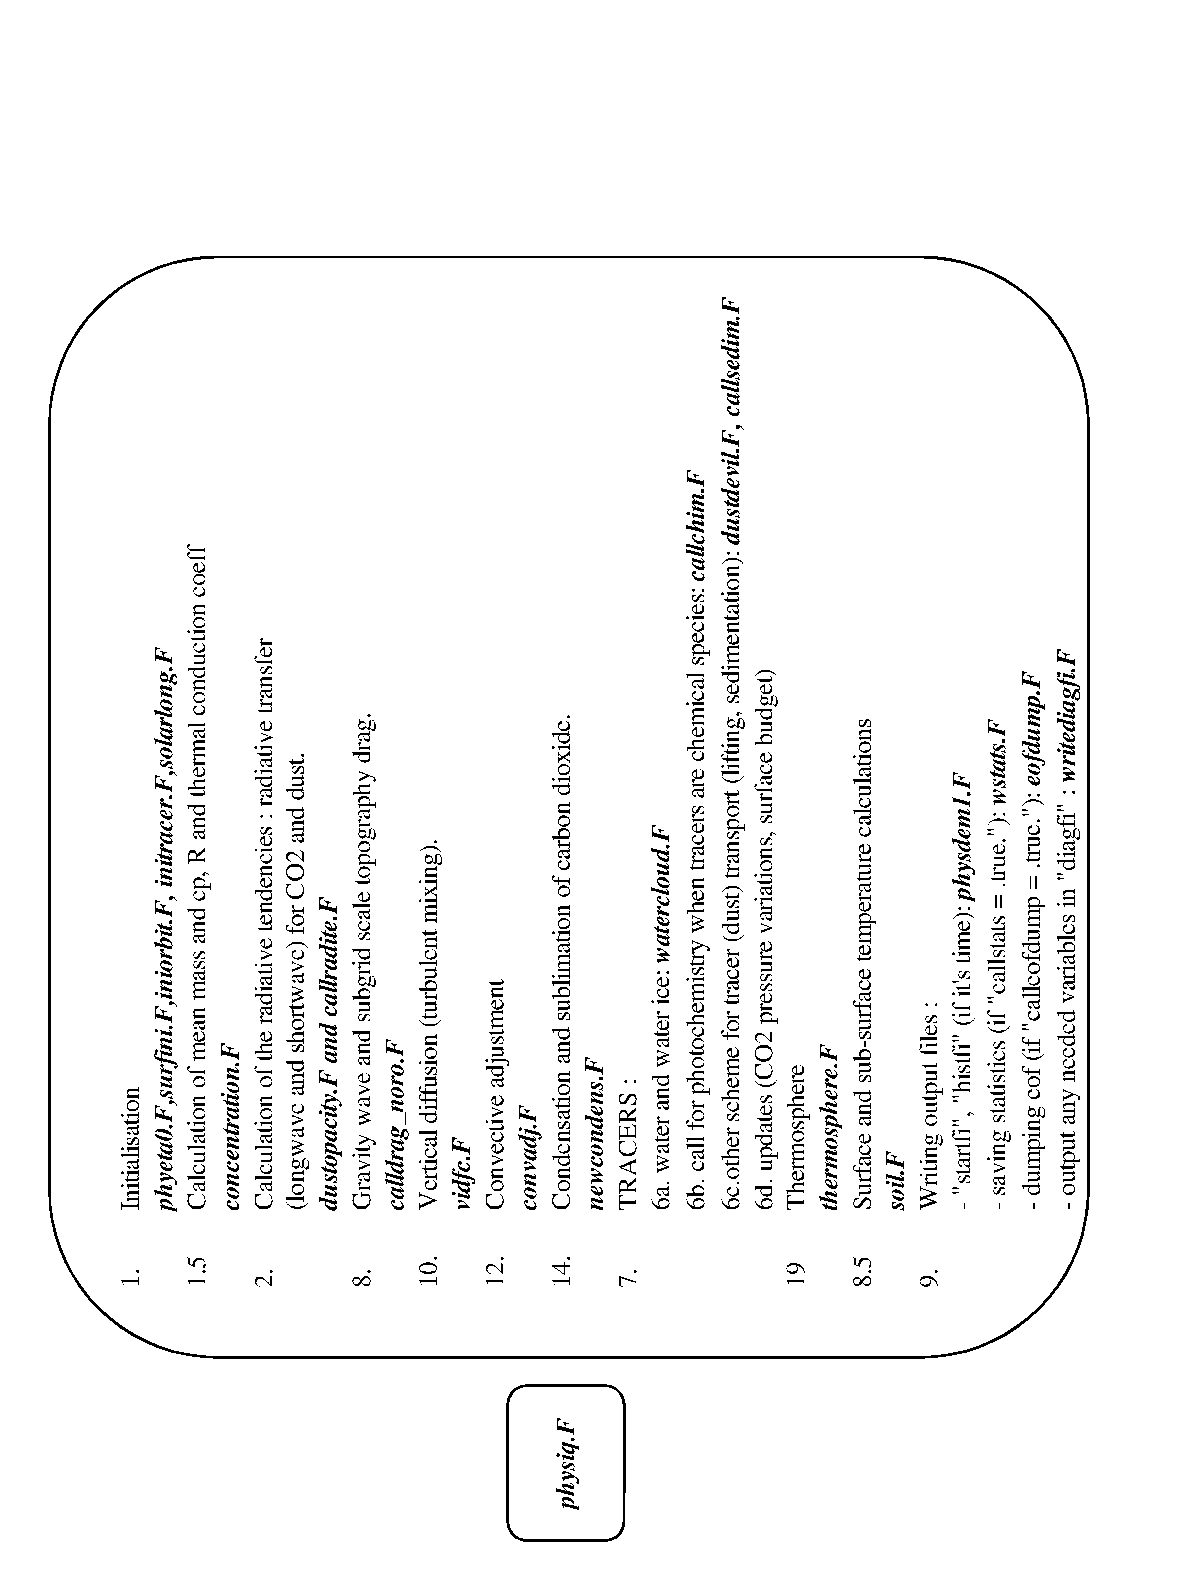
\includegraphics[scale=0.70,angle=-90]{Fig/physique.eps}
\caption{Organigram of subroutine function physiq.F90}
\label{fg:organi_phys}
\end{flushleft}
\end{figure}


%%%%%%%%%%%%%%%%%%%%%%%%%%%%%%%%%%%%%%%%%%%%%%%%%%
%  Compilation du modele
%%%%%%%%%%%%%%%%%%%%%%%%%%%%%%%%%%%%%%%%%%%%%%%%%%

\section{Compiling the model}
\index{Compiling the model}

\label{sc:compil1}
Technically, the model is compiled using the Unix utility {\tt make}.
The file {\tt makefile}, which describes the code dependencies
and requirements,
is created automatically by the script
\begin{verbatim}
create_make_gcm
\end{verbatim}
This utility script recreates the {\tt makefile} file when necessary,
for example, when a source file has been added or removed since the last
compilation.

{\bf None of this is visible to the user.
To compile the model just run the command}
\begin{verbatim}
makegcm
\end{verbatim}
with adequate options (e.g. {\tt makegcm -d 62x48x32 -p mars gcm}), as
discussed below and described in section~\ref{sc:run1}.


The {\tt makegcm} command compiles the model ({\bf gcm}) and related utilities
({\bf newstart}, {\bf start2archive}, {\bf testphys1d}).
A detailed description of how to use it and of the various parameters that
can be supplied
is given in the help manual below
(which will also be given by the \verb+makegcm -h+ command).\\
Note that before compiling the GCM with {\tt makegcm} you should have set
the environment variable {\bf LIBOGCM} to a path where intermediate
objects and libraries will be generated.\\
If using Csh:
\begin{verbatim}
setenv  LIBOGCM /where/you/want/objects/to/go/libo
\end{verbatim}
If using Bash:
\begin{verbatim}
export  LIBOGCM=/where/you/want/objects/to/go/libo
\end{verbatim}
\paragraph{Help manual for the makegcm script}
%%%%%%%%%%%%%%%%%%%%%%%%%%%%%%%%%%%%%%%%%%%%%%%%%%%%%%%
% makegcm.help:  lu dans makegcm
%%%%%%%%%%%%%%%%%%%%%%%%%%%%%%%%%%%%%%%%%%%%%%%%%%%%%%%
{\footnotesize
\begin{verbatim}
makegcm [Options] prog


The makegcm script:
-------------------

1. compiles a series of subroutines located in the $LMDGCM/libf
 sub-directories.
 The objects are then stored in the libraries in $LIBOGCM.

2. then, makegcm compiles program prog.f located by default in
$LMDGCM/libf/dyn3d and makes the link with the libraries.

Environment Variables '$LMDGCM' and '$LIBOGCM'
 must be set as environment variables or directly
 in the makegcm file.

The makegcm command is used to control the different versions of the model
 in parallel, compiled using the compilation options 
 and the various dimensions, without having to recompile the whole model.

The FORTRAN libraries are stored in directory $LIBOGCM.


OPTIONS:
--------

The following options can either be defined by default by editing the
makegcm "script", or in interactive mode:

-d imxjmxlm  where im, jm, and lm are the number of longitudes,
             latitudes and vertical layers respectively.

-t ntrac   Selects the number of tracers present in the model

             Options -d and -t overwrite file 
             $LMDGCM/libf/grid/dimensions.h
             which contains the 3 dimensions of the
             horizontal grid 
             im, jm, lm plus the number of tracers passively advected
             by the dynamics ntrac,
             in 4 PARAMETER FORTRAN format 
             with a new file:
             $LMDGCM/libf/grid/dimension/dimensions.im.jm.lm.tntrac
             If the file does not exist already
             it is created by the script
             $LMDGCM/libf/grid/dimension/makdim

-p PHYS    Selects the set of physical parameterizations
           you want to compile the model with.
           The model is then compiled using the physical
           parameterization sources in directory:
            $LMDGCM/libf/phyPHYS

-g grille  Selects the grid type.
           This option overwrites file
           $LMDGCM/libf/grid/fxyprim.h
           with file
           $LMDGCM/libf/grid/fxy_grille.h
           the grid can take the following values:
           1. reg - the regular grid
           2. sin - to obtain equidistant points in terms of sin(latitude)
           3. new - to zoom into a part of the globe

-O "compilation options" set of fortran compilation options to use

-include path
           Used if the subroutines contain #include files (ccp) that 
           are located in directories that are not referenced by default.

-adjnt     Compiles the adjoint model to the dynamical code.

-filtre  filter
           To select the longitudinal filter in the polar regions.
           "filter" corresponds to the name of a directory located in
           $LMDGCM/libf. The standard filter for the model is "filtrez"
           which can be used for a regular grid and for a  
           grid with longitudinal zoom.

-link "-Ldir1 -lfile1 -Ldir2 -lfile2 ..."
           Adds a link to FORTRAN libraries
           libfile1.a, libfile2.a ... 
           located in directories dir1, dir2 ...respectively
           If dirn is a directory with an automatic path 
           (/usr/lib ... for example) 
           there is no need to specify  -Ldirn.

\end{verbatim}
}

%%%%%%%%%%%%%%%%%%%%%%%%%%%%%%%%%%%%%%%%%%%%%%%%%%%%%%%

\chapter{Input/Output}
\label{sc:io}

\section{NetCDF format}

%%%%%%%%%%%%%%%%%%%%%%%%%%
GCM input/output data are written in {\bf NetCDF} format
(Network Common Data Form). NetCDF is an interface used to store and access
geophysical data, and a library that provides an implementation of this
interface. The NetCDF library also defines a machine-independent format for
representing scientific data. 
Together, the interface, library and format support the creation, access and
sharing of scientific data. NetCDF was developed at the Unidata Program Center
in Boulder, Colorado. The freely available source can be obtained from
the Unidata website:
\begin{verbatim}
http://www.unidata.ucar.edu/software/netcdf
\end{verbatim}


%%%%%%%%%%%%%%%%%%%%%%%%%%

A data set in NetCDF format is a single file, as it is self-descriptive.

\subsection{NetCDF text representation: ncdump}

This utility is included in the NetCDF library.
It generates the CDL representation (text format of the file content) to the standard output
from the NetCDF file specified as input. 

\paragraph{Main options for the ncdump command}

\begin{center}
{\it ncdump diagfi.nc}
\end{center}

\noindent
dump contents of NetCDF file {\tt diagfi.nc} to standard output
(i.e. the screen).

\begin{center}
{\it ncdump -c diagfi.nc}
\end{center}

\noindent
Displays the {\bf coordinate} variable values (variables which are also
dimensions), as well as the declarations, variables and attribute values.
The values of the non-coordinate variable data are not displayed at
the output.

\begin{center}
{\it ncdump -h diagfi.nc}
\end{center}

\noindent
Shows only the informative header of the file, which is the declaration
of the dimensions, variables and attributes, but not the values of these
variables. The output is identical to that in option {\bf -c} except for
the fact that the coordinated variable values are not included.

\begin{center}
{\it ncdump -v var1,...,varn diagfi.nc}
\end{center}

\noindent
The output includes the specific variable values,
as well as all the dimensions, variables and attributes.
More that one variable can be specified in the list following this option.
The list must be a simple argument for the command, and must not contain any
spaces. If no variable is specified, the command displays all the values of
the variables in the file by default.  


\subsection{Graphic visualization of NetCDF files using GrAds}

GrAdS (The Grid Analysis and Display System) is a graphic software developed
by Brian Doty at the "Center for Ocean-Land-Atmosphere (COLA)".

One of its functions is to enable data stored in NetCDF format to be
visualized directly. In figure~\ref{fg:grads} for example, we can see the
GrADS visualization of the temperature data at a given moment.
%
\begin{figure}
\centering
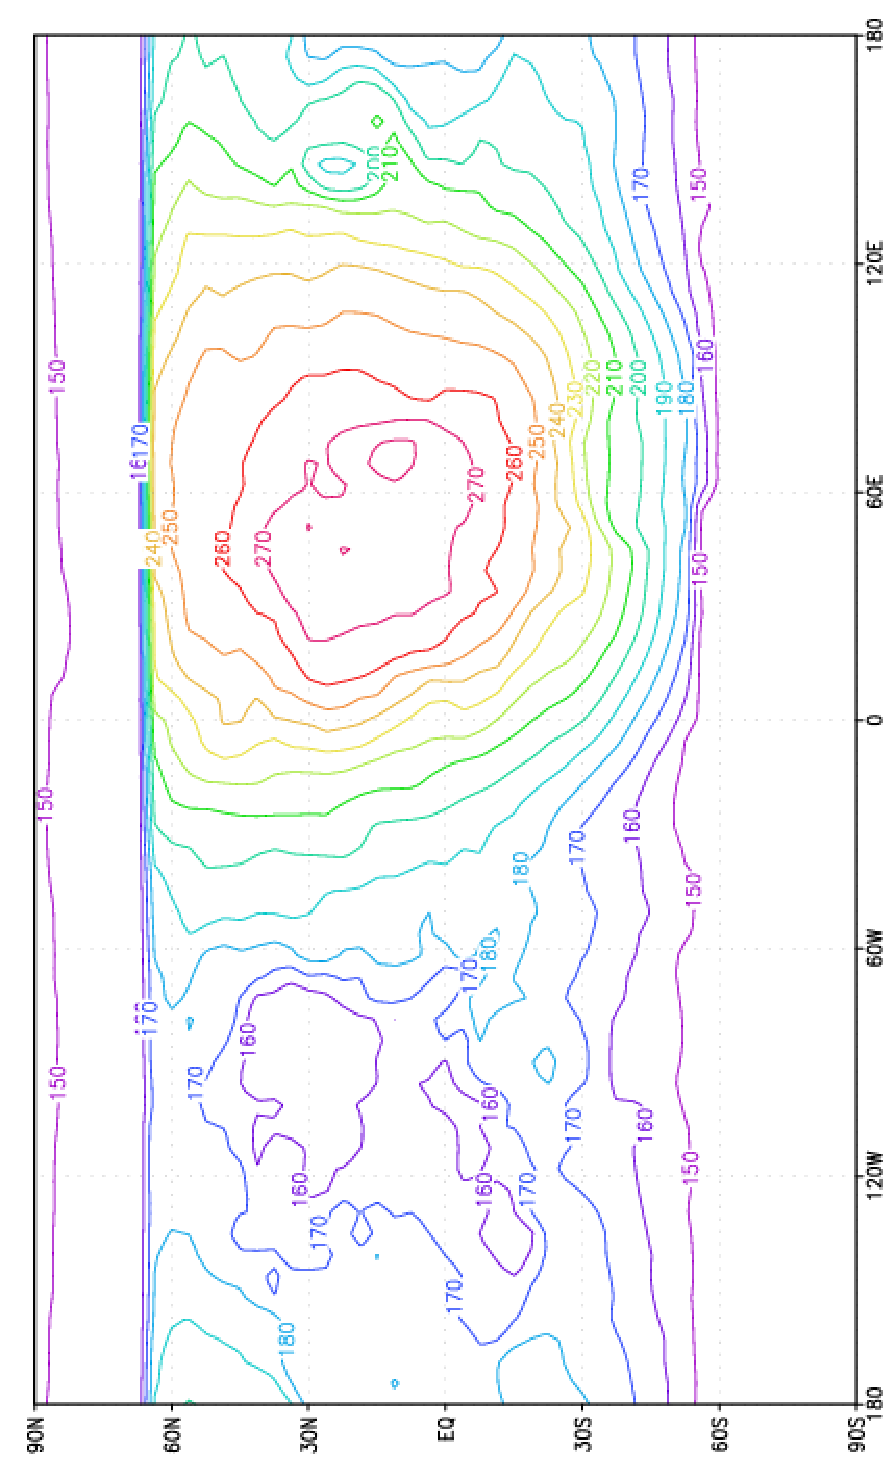
\includegraphics[width=0.5\textwidth,angle=270]{Fig/grads.pdf}
\caption{Example of temperature data at a given time using
GrADS visualization\label{fg:grads}}
\end{figure}
%
However, unlike NetCDF, GrADS only recognizes files where all the variables are stored on the same horizontal grid.
These variables can be in 1, 2, 3 or 4 dimensions (X,Y,Z and t).\\

GrADS can also be obtained from:
\begin{verbatim}
http://grads.iges.org/grads/
\end{verbatim}

\subsection{Graphic visualization of NetCDF files using Ferret}

Ferret may also be used to visualize the contents of NetCDF files. Download intruction and documentation are available from the official website:
\begin{verbatim}
https://ferret.pmel.noaa.gov/Ferret/
\end{verbatim} 

\section{Input and parameter files}

%{\bf \it Examples of initialization files can be found in directory
%\begin{verbatim}$PATH1/LMDZ.MARS/deftank \end{verbatim}}
\label{loc:entrees}

The (3D version of the) GCM requires
the input of two initialization files (in NetCDF format):\\
-{\bf start.nc}
contains the initial states of the dynamical variables.\\
-{\bf startfi.nc}
contains the initial states of the physical variables.\\
Note that collections of initial states can be retreived at:\\
\verb+http://www.lmd.jussieu.fr/~lmdz/planets/mars/starts+ \\
Extracting {\tt start.nc} and {\tt startfi.nc} from these archived
requires using program {\tt newstart}, as described in
section~\ref{sc:newstart}.\\

\noindent
To run, the GCM also requires the  four following
parameter files (ascii text files):\\
-{\bf run.def} the parameters of the dynamical part of the program,
and the temporal integration of the model.\\
-{\bf callphys.def} the parameters for calling the physical part.\\
-{\bf traceur.def} the names of the tracer to use.\\
-{\bf z2sig.def}
 the vertical distribution of the atmospheric layers.\\
Examples of these parameter files can be found in the
\verb+LMDZ.MARS/deftank+ directory.

\subsection{run.def}
\label{vb:run.def}
%%%%%%%%%%%%%%%%%%%%%%%%%%%%%%%%%%%%%%%%%%%%%%%%%%%%%%%
% run.def: les param sont lus dans dyn3d/defrun.F
%%%%%%%%%%%%%%%%%%%%%%%%%%%%%%%%%%%%%%%%%%%%%%%%%%%%%%%

A typical {\tt run.def} file is given as an example below.
The choice of variables to be set is simple (e.g.
 {\tt nday} number of modeled days to run),
while the others do not need to be changed for normal use.\\
The format of the {\tt run.def} file is quite straightforward
(and flexible): values given to parameters must be given as:
\begin{verbatim}
  parameter = value
\end{verbatim}
Any blank line or line beginning with symbol {\bf \#} is
a comment, and instruction lines may be written in any order.
Moreover, not specifying a parameter/value set (e.g. deleting it
or commenting it out) means you want the GCM to use a default built-in value.
Additionally, one may use a specific keyword {\bf INCLUDEDEF} to specify
another (text) file in which to also read values of parameters; e.g.:
\begin{verbatim}
INCLUDEDEF=callphys.def
\end{verbatim}


\noindent Here are some details about some of the parameters which may be
set in {\tt run.def}:
\begin{itemize}
\item {\bf day\_step}, the number of dynamical steps per day to use for
the time integration. This needs to be large enough for the model
to remain stable (this is related to the CFL stability criterion
which essentially depends on the horizontal resolution of the model).
On Mars, in theory, the GCM can run with
{\tt day\_step}=480 using the 64$\times$48 grid, but model stability
improves when this number is higher: {\tt day\_step}=960 is recommended
 when using the 64$\times$48 grid. According to the CFL criterion,
{\tt day\_step} should vary in proportion with the resolution: for example
{\tt day\_step}=480 using the 32$\times$24 horizontal resolution.
Note that {\tt day\_step} must also be divisible by {\tt iperiod}.

\item {\bf tetagdiv, tetagrot, tetatemp} control the dissipation intensity.
It is better to limit the dissipation intensity
(tetagdiv, tetagrot, tetatemp should not be too low).
However the model diverges if tetagdiv, tetagrot, tetatemp are too high,
especially if there is a lot of dust in the atmosphere. \\
Example used with nitergdiv=1 and  nitergrot=niterh=2 : \\
- using the 32$\times$24 grid tetagdiv=6000~s ; tetagrot=tetatemp=30000~s \\
- using the 64$\times$48 grid: tetagdiv=2500~s ; tetagrot=tetatemp=5000~s

\item {\bf idissip} is the time step used for the dissipation:
dissipation is computed and added every {\tt idissip} dynamical
time step. If {\tt idissip} is
too short, the model waste time in these calculations. But if idissip is too
long, the  dissipation will not be parametrized correctly and the  model will
be more likely to diverge. 
A check must be made, so that:
{\tt idissip}~$<$~{\tt tetagdiv}$\times${\tt daystep}/88775
(same rule for {\tt tetagrot} and {\tt tetatemp}).
This is tested automatically during the run.

\item {\bf iphysiq} is the time step used for the physics:
physical tendencies are computed every {\tt iphysiq} dynamical time step.
In practice, we
usually set the physical time step to be of the order of half an hour. 
We thus generally set {\tt iphysiq}= {\tt day\_step}/48

\end{itemize}

\noindent
{\it Example of run.def file: }
{\footnotesize
{\footnotesize
\begin{verbatim}

#------------------------------
# Parametres de controle du run
#------------------------------

# Nombre de jours d'integration
     nday=669

# nombre de pas par jour (multiple de iperiod) ( ici pour  dt = 1 min )
 day_step = 960

# periode pour le pas Matsuno (en pas)
  iperiod=5

# periode de sortie des variables de controle (en pas)
  iconser=120

# periode d'ecriture du fichier histoire (en jour)
    iecri=100

# periode de stockage fichier histmoy (en jour)
 periodav=60.

# periode de la dissipation (en pas)
  idissip=5

# choix de l'operateur de dissipation (star ou  non star )
 lstardis=.true.

# avec ou sans coordonnee hybrides
 hybrid=.true.

# nombre d'iterations de l'operateur de dissipation   gradiv
nitergdiv=1

# nombre d'iterations de l'operateur de dissipation  nxgradrot
nitergrot=2

# nombre d'iterations de l'operateur de dissipation  divgrad
   niterh=2

# temps de dissipation des plus petites long.d ondes pour u,v (gradiv)
 tetagdiv=10000.

# temps de dissipation des plus petites long.d ondes pour u,v(nxgradrot)
 tetagrot=10000.

# temps de dissipation des plus petites long.d ondes pour  h ( divgrad)
 tetatemp=10000.

# coefficient pour gamdissip
  coefdis=0.

# choix du shema d'integration temporelle (Matsuno ou Matsuno-leapfrog)
  purmats=.false.

# avec ou sans physique
   physic=.true.

# periode de la physique (en pas)
  iphysiq=20

# choix d'une grille reguliere
  grireg=.true.

# frequence (en pas) de l'ecriture du fichier diagfi
 ecritphy=1920

# longitude en degres du centre du zoom
   clon=63.

# latitude en degres du centre du zoom
   clat=0.

# facteur de grossissement du zoom,selon longitude
  grossismx=1.

# facteur de grossissement du zoom ,selon latitude
 grossismy=1.

#  Fonction  f(y)  hyperbolique  si = .true.  , sinon  sinusoidale
  fxyhypb=.false.

# extension en longitude  de la zone du zoom  ( fraction de la zone totale)
   dzoomx= 0.

# extension en latitude de la zone  du zoom  ( fraction de la zone totale)
   dzoomy=0.

#  raideur du zoom en  X
    taux=2.

#  raideur du zoom en  Y
    tauy=2.

#  Fonction  f(y) avec y = Sin(latit.) si = .TRUE. ,  Sinon  y = latit.
  ysinus= .false.

# Avec sponge layer
  callsponge  = .true.

# Sponge:  mode0(u=v=0), mode1(u=umoy,v=0), mode2(u=umoy,v=vmoy)
  mode_sponge= 2

# Sponge:  hauteur de sponge (km)
  hsponge= 90

# Sponge:  tetasponge (secondes)
  tetasponge = 50000

# some definitions for the physics, in file 'callphys.def'
INCLUDEDEF=callphys.def


\end{verbatim}
}

}
%%%%%%%%%%%%%%%%%%%%%%%%%%%%%%%%%%%%%%%%%%%%%%%%%%%%%%%


\subsection{callphys.def}
\label{sc:callphys.def}
%%%%%%%%%%%%%%%%%%%%%%%%%%%%%%%%%%%%%%%%%%%%%%%%%%%%%%%
% callphys.def: les param sont lus dans phymars/inifis.F
%%%%%%%%%%%%%%%%%%%%%%%%%%%%%%%%%%%%%%%%%%%%%%%%%%%%%%%
The {\tt callphys.def} file (along the same format
as the {\tt run.def} file) contains parameter/value sets
for the physics.\\

 
\noindent
{\it Example of callphys.def file: }
{\footnotesize
{\footnotesize
\begin{verbatim}

## Orbit / general options
## ~~~~~~~~~~~~~~~~~~~~~~~
# Run with or without tracer transport ?
tracer    = .true.
# Diurnal cycle ?  if diurnal=false, diurnally averaged solar heating
diurnal   = .true.
# Seasonal cycle ? if season=false, Ls stays constant, to value set in "start"
season    = .true.
# Tidally resonant orbit ? must have diurnal=false, correct rotation rate in newstart
tlocked   = .false.
# Tidal resonance ratio ? ratio T_orbit to T_rotation
nres      = 10
# Write some more output on the screen ?
lwrite    = .false.
# Save statistics in file "stats.nc" ?
callstats = .true.
# Test energy conservation of model physics ?
enertest  = .true.

## Radiative transfer options
## ~~~~~~~~~~~~~~~~~~~~~~~~~~
# call radiative transfer?
callrad    = .true.
# the rad. transfer is computed every "iradia" physical timestep
iradia     = 4
# call multilayer correlated-k radiative transfer ?
corrk      = .true.
# folder in which correlated-k data is stored ?
corrkdir   = CO2_H2Ovar
# call visible gaseous absorption in radiative transfer ?
callgasvis = .true.
# Include Rayleigh scattering in the visible ?
rayleigh   = .true.
# Characteristic planetary equilibrium (black body) temperature
# This is used only in the aerosol radiative transfer setup. (see aerave.F)
tplanet    = 215.
# Output spectral OLR in 1D/3D?
specOLR    = .false.
# Output global radiative balance in file 'rad_bal.out' - slow for 1D!!
meanOLR    = .true.
# Variable gas species: Radiatively active ?
varactive  = .true.
# Variable gas species: Fixed vertical distribution ?
varfixed   = .false.
# Variable gas species: Saturation percentage value at ground ?
satval     = 0.0

## Star type
## ~~~~~~~~~
startype = 1
# ~~~~~~~~~~~~~~~~~~~~~~~~~~~~~~~~~~~~~~~~~~~~~~~~~~~~~~~~~~
# The choices are:
#
#	startype = 1		Sol        (G2V-class main sequence)
#	startype = 2		Ad Leo     (M-class, synthetic)
#   startype = 3        GJ644
#   startype = 4        HD128167
# ~~~~~~~~~~~~~~~~~~~~~~~~~~~~~~~~~~~~~~~~~~~~~~~~~~~~~~~~~~~
# Stellar flux at 1 AU. Examples:
# 1366.0 W m-2		Sol today
# 1024.5 W m-2		Sol today x 0.75 = weak early Sun
# 18.462 W m-2		The feeble Gl581
# 19.960 W m-2		Gl581 with e=0.38 orbital average
Fat1AU = 1024.5

## Tracer and aerosol options
## ~~~~~~~~~~~~~~~~~~~~~~~~~~
# Gravitational sedimentation of tracers (KEEP FALSE FOR NOW) ?
sedimentation = .false.

## Other physics options
## ~~~~~~~~~~~~~~~~~~~~~
# call turbulent vertical diffusion ?
calldifv = .true.
# call convective adjustment ?
calladj  = .true.
# call thermal conduction in the soil ?
callsoil = .true.

#########################################
## extra specific options for Early Mars
#########################################

## Tracer and aerosol options
## ~~~~~~~~~~~~~~~~~~~~~~~~~~
# Fixed aerosol distributions?
aerofixed     = .false.
# Varying H2O cloud fraction?
CLFvarying    = .false.
# H2O cloud fraction?
CLFfixval     = 0.5
# number mixing ratio of CO2 ice particles
Nmix_co2      = 100000.
# number mixing ratio of water ice particles
Nmix_h2o      = 100000.

## Water options
## ~~~~~~~~~~~~~
# Model water cycle
water         = .true.
# Model water cloud formation
watercond     = .true.
# Model water precipitation (including coagulation etc.)
waterrain     = .true.
# WATER: Precipitation threshold (simple scheme only) ?
rainthreshold = 0.0011
# Include hydrology ?
hydrology     = .true.
# H2O snow (and ice) albedo ?
albedosnow    = 0.5
# Maximum sea ice thickness ?
maxicethick   = 0.05
# Freezing point of seawater (degrees C) ?
Tsaldiff      = 0.0

## CO2 options
## ~~~~~~~~~~~
# gas is non-ideal CO2 ?
nonideal      = .false.
# call CO2 condensation ?
co2cond       = .true.
# Set initial temperature profile to 1 K above CO2 condensation everywhere?
nearco2cond   = .false.

\end{verbatim}
}

}
%%%%%%%%%%%%%%%%%%%%%%%%%%%%%%%%%%%%%%%%%%%%%%%%%%%%%%%

\subsection{traceur.def}
\label{sc:traceur.def}
Tracers in input ({\tt start.nc} and {\tt startfi.nc}) and output
files ({\tt restart.nc} and {\tt restartfi.nc}) are stored using
individual tracer names (e.g. {\tt co2} for CO2 gas, {\tt h2o\_vap}
for water vapour, {\tt h2o\_ice} for water ice, ...).\\
The first line of the {\tt traceur.def} file (an ASCII file) must
contain the number of tracers to load and use (this number should
be the same as given to the {\tt -t} option of the {\tt makegcm}
script when the GCM was compiled), followed by the tracer names
(one per line). Note that if the corresponding tracers are not
found in input files {\tt start.nc} and {\tt startfi.nc}, then the
tracer is initialized to zero.\\


\noindent {\it Example of a traceur.def file}:
with CO2, dust distribution moments, (water ice) cloud condensation nuclei moments, water vapour and water ice tracers
{\footnotesize
\begin{verbatim}
7
co2
dust_number
dust_mass
ccn_number
ccn_mass
h2o_ice
h2o_vap
\end{verbatim}
}

\subsection{z2sig.def}
The {\tt Z2sig.def} file contains the pseudo-altitudes
(in km) at which the user wants to set the vertical levels.\\
Note that levels should be unevenly spread, with a higher resolution
near the surface in order to capture the rapid variations of variables
there. It is recommended to use the altitude levels as set in the
{\tt z2sig.def} file provided in the {\tt deftank} directory.\\


\noindent
{\it Example of  z2sig.def file
(this version for 49 layers between  0 and 300~km):}
{\footnotesize
\begin{verbatim}
10.00000     H: atmospheric scale height (km) (used as a reference only)
0.0040       Typical pseudo-altitude (m) for 1st layer (z=H*log(sigma))
0.018       ,, ,,  ,, ,, ,, ,,  ,, ,, ,,  2nd layer, etc...
0.0400
0.1000
0.228200
0.460400
0.907000
1.73630
3.19040
5.54010
8.97780
13.5138
18.9666
25.0626
31.5527
38.4369
45.4369
52.4369
\end{verbatim}

}

\subsection{Initialization files: start and startfi}

%
\begin{figure}[h]
\centering
\framebox[0.8\textwidth][c]{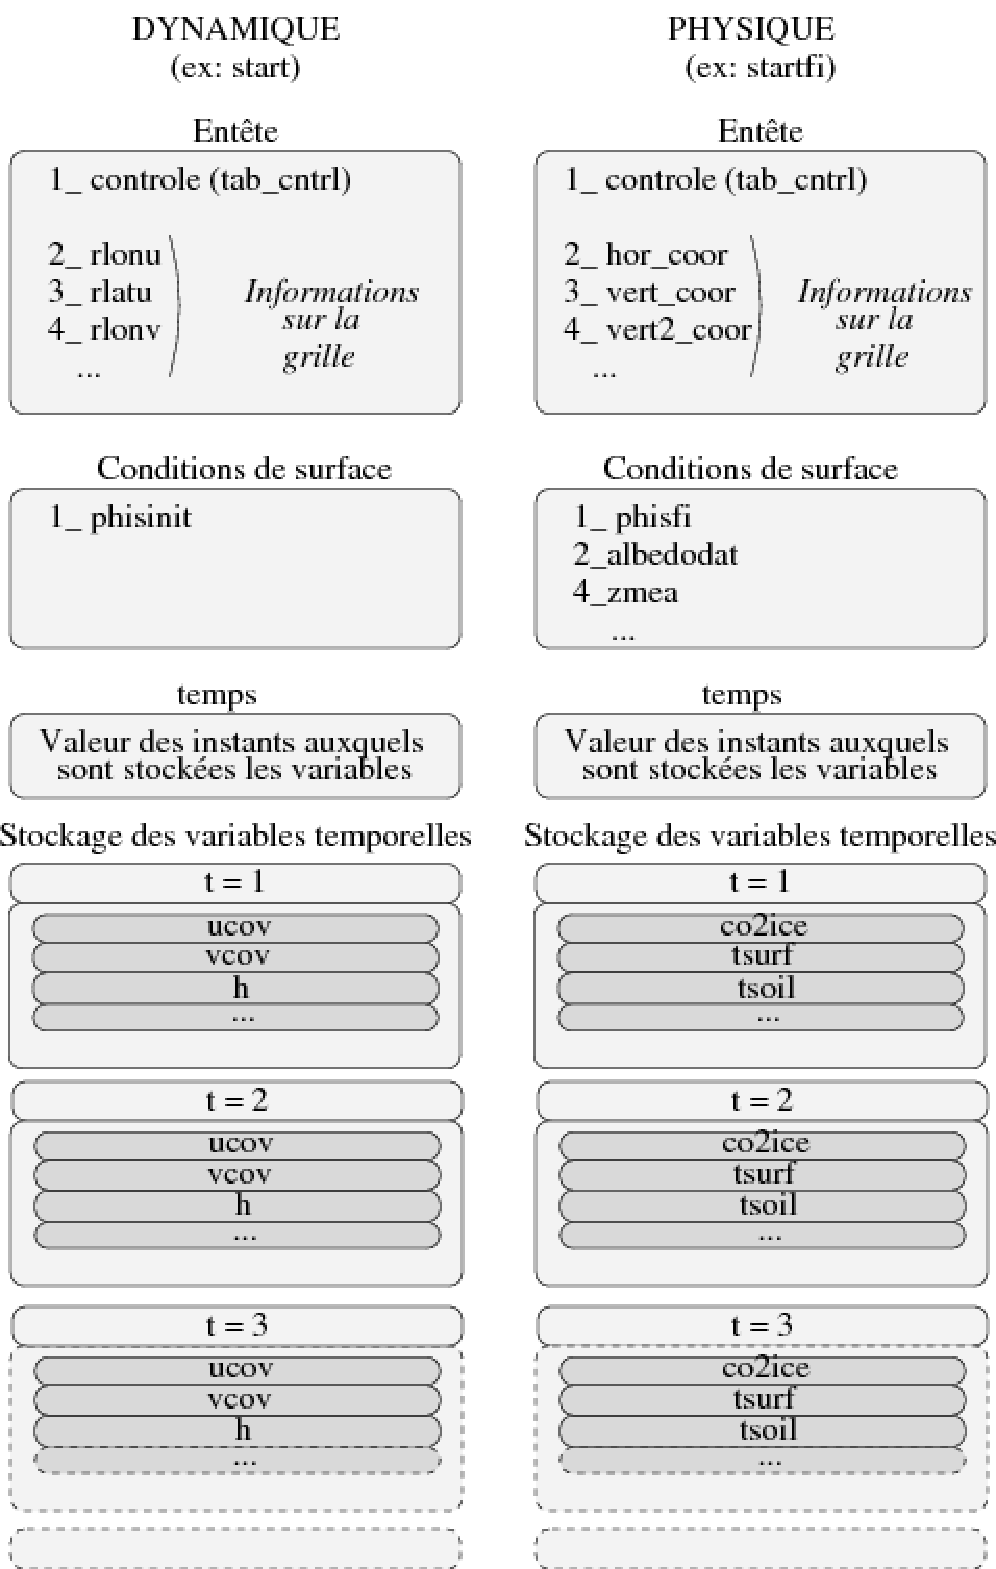
\includegraphics[width=0.7\textwidth]{Fig/netcdf.pdf}}
\caption{Organization of NetCDF files \label{fg:netcdf}}
\end{figure}
%
Files {\tt start.nc} and {\tt startfi.nc}, like all the NetCDF files of
the GCM,
are constructed on the same model (see NetCDF file composition,
figure~\ref{fg:netcdf}). They contain:\\
- a header with a ``control'' variable followed by a series of variables
defining the (physical and dynamical) grids \\
- a series of non temporal variables that give information about surface 
conditions on the planet.\\
- a ``time'' variable giving the values of the different instants at which 
the temporal variables are stored 
(a single time value (t=0) for start,
as it describes the dynamical initial states,
and no time values for startfi, as it describes only a physical state).\\

To dump (in text format) the contents of a {\tt start.nc} file using the
{\tt ncdump} command:\\

\noindent
{\it ncdump -h start.nc}\\
%%%%%%%%%%%%%%%%%%%%%%%%%%%%%%%%%%%%%%%%%%%%%%%%%%%%%%%
% List START
%%%%%%%%%%%%%%%%%%%%%%%%%%%%%%%%%%%%%%%%%%%%%%%%%%%%%%%
{\footnotesize
\begin{verbatim}
netcdf start {
dimensions:
        index = 100 ;
        rlonu = 33 ;
        latitude = 25 ;
        longitude = 33 ;
        rlatv = 24 ;
        altitude = 18 ;
        interlayer = 19 ;
        Time = UNLIMITED ; // (1 currently)
variables:
        float controle(index) ;
                controle:title = "Parametres de controle" ;
        float rlonu(rlonu) ;
                rlonu:title = "Longitudes des points U" ;
        float rlatu(latitude) ;
                rlatu:title = "Latitudes des points U" ;
        float rlonv(longitude) ;
                rlonv:title = "Longitudes des points V" ;
        float rlatv(rlatv) ;
                rlatv:title = "Latitudes des points V" ;
        float ap(interlayer) ;
                ap:title = "Coef A: hybrid pressure levels" ;
        float bp(interlayer) ;
                bp:title = "Coef B: hybrid sigma levels" ;
        float aps(altitude) ;
                aps:title = "Coef AS: hybrid pressure at midlayers" ;
        float bps(altitude) ;
                bps:title = "Coef BS: hybrid sigma at midlayers" ;
        float presnivs(altitude) ;
        float latitude(latitude) ;
                latitude:units = "degrees_north" ;
                latitude:long_name = "North latitude" ;
        float longitude(longitude) ;
                longitude:long_name = "East longitude" ;
                longitude:units = "degrees_east" ;
        float altitude(altitude) ;
                altitude:long_name = "pseudo-alt" ;
                altitude:units = "km" ;
                altitude:positive = "up" ;
        float cu(latitude, rlonu) ;
                cu:title = "Coefficient de passage pour U" ;
        float cv(rlatv, longitude) ;
                cv:title = "Coefficient de passage pour V" ;
        float aire(latitude, longitude) ;
                aire:title = "Aires de chaque maille" ;
        float phisinit(latitude, longitude) ;
                phisinit:title = "Geopotentiel au sol" ;
        float Time(Time) ;
                Time:title = "Temps de simulation" ;
                Time:units = "days since    1-01-01 00:00:00" ;
        float ucov(Time, altitude, latitude, rlonu) ;
                ucov:title = "Vitesse U" ;
        float vcov(Time, altitude, rlatv, longitude) ;
                vcov:title = "Vitesse V" ;
        float teta(Time, altitude, latitude, longitude) ;
                teta:title = "Temperature" ;
        float h2o_ice(Time, altitude, latitude, longitude) ;
                h2o_ice:title = "Traceur h2o_ice" ;
        float h2o_vap(Time, altitude, latitude, longitude) ;
                h2o_vap:title = "Traceur h2o_vap" ;
        float masse(Time, altitude, latitude, longitude) ;
                masse:title = "C est quoi ?" ;
        float ps(Time, latitude, longitude) ;
                ps:title = "Pression au sol" ;

// global attributes:
                :title = "Dynamic start file" ;
}
\end{verbatim}
}

%%%%%%%%%%%%%%%%%%%%%%%%%%%%%%%%%%%%%%%%%%%%%%%%%%%%%%%

\noindent
List of contents of a {\tt startfi.nc} file:\\

\noindent
{\it ncdump -h startfi.nc}\\
%%%%%%%%%%%%%%%%%%%%%%%%%%%%%%%%%%%%%%%%%%%%%%%%%%%%%%%
% List startfi
%%%%%%%%%%%%%%%%%%%%%%%%%%%%%%%%%%%%%%%%%%%%%%%%%%%%%%%
{\footnotesize
\begin{verbatim}
netcdf startfi {
dimensions:
        index = 100 ;
        physical_points = 738 ;
        subsurface_layers = 18 ;
        nlayer_plus_1 = 19 ;
        number_of_advected_fields = 3 ;
variables:
        float controle(index) ;
                controle:title = "Control parameters" ;
        float soildepth(subsurface_layers) ;
                soildepth:title = "Soil mid-layer depth" ;
        float longitude(physical_points) ;
                longitude:title = "Longitudes of physics grid" ;
        float latitude(physical_points) ;
                latitude:title = "Latitudes of physics grid" ;
        float area(physical_points) ;
                area:title = "Mesh area" ;
        float phisfi(physical_points) ;
                phisfi:title = "Geopotential at the surface" ;
        float albedodat(physical_points) ;
                albedodat:title = "Albedo of bare ground" ;
        float ZMEA(physical_points) ;
                ZMEA:title = "Relief: mean relief" ;
        float ZSTD(physical_points) ;
                ZSTD:title = "Relief: standard deviation" ;
        float ZSIG(physical_points) ;
                ZSIG:title = "Relief: sigma parameter" ;
        float ZGAM(physical_points) ;
                ZGAM:title = "Relief: gamma parameter" ;
        float ZTHE(physical_points) ;
                ZTHE:title = "Relief: theta parameter" ;
        float co2ice(physical_points) ;
                co2_ice:title = "CO2 ice cover" ;
        float inertiedat(subsurface_layers, physical_points) ;
                inertiedat:title = "Soil thermal inertia" ;
        float tsurf(physical_points) ;
                tsurf:title = "Surface temperature" ;
        float tsoil(subsurface_layers, physical_points) ;
                tsoil:title = "Soil temperature" ;
        float emis(physical_points) ;
                emis:title = "Surface emissivity" ;
        float q2(nlayer_plus_1, physical_points) ;
                q2:title = "pbl wind variance" ;
        float h2o_ice(physical_points) ;
                h2o_ice:title = "tracer on surface" ;

// global attributes:
                :title = "Physics start file" ;
}
\end{verbatim}
}

%%%%%%%%%%%%%%%%%%%%%%%%%%%%%%%%%%%%%%%%%%%%%%%%%%%%%%%



%%%%%%%%%%%%%%%%%%%%%%%%%%%%%%%%%%%%%%%%%%%%%%%%%%%%%%%
%    Description des start et startfi
%%%%%%%%%%%%%%%%%%%%%%%%%%%%%%%%%%%%%%%%%%%%%%%%%%%%%%%

\paragraph{Physical and dynamical headers}

There are two types of headers: one for the physical headers,
and one for the dynamical headers.
The headers always begin with a ``control' variable
(described below), that is allocated differently in the physical and
dynamical parts.
The other variables in the header concern the (physical and dynamical) grids.
They are the following:\\

\noindent
the horizontal coordinates\\
- {\bf rlonu}, {\bf rlatu}, {\bf rlonv}, {\bf rlatv} for the dynamical part,\\
- {\bf lati}, {\bf long} for the physical part,\\

\noindent
the coefficients for passing from the physical grid to the dynamical grid\\
- {\bf cu},{\bf cv} only in the dynamical header\\

\noindent
and finally, the grid box areas\\
- {\bf aire} for the dynamical part,\\
- {\bf area} for the physical part.\\

\paragraph{Surface conditions}

The surface conditions are mostly given in the physical NetCDF files by
variables:\\
- {\bf phisfi} for the initial state of surface geopotential,\\
- {\bf albedodat} for the bare ground albedo,\\
- {\bf inertiedat} for the surface thermal inertia,\\
- {\bf zmea}, {\bf zstd}, {\bf zsig}, {\bf zgam} and {\bf zthe} for
  the subgrid scale topography.\\

\noindent
For the dynamics:\\
- {\bf physinit} for the initial state of surface geopotential\\

\noindent
Remark: variables {\bf phisfi} and {\bf physinit} contain the same information
(surface geopotential), but {\bf phisfi} gives the geopotential values on the
physical grid, while {\bf physinit} give the values on the dynamical grid.\\

\paragraph{Physical and dynamical state variables}
To save disk space, the initialization files store the variables used by
the model, rather than the ``natural'' variables.\\

\noindent
For the dynamics:
\begin{description}
\item - {\bf ucov} and {\bf vcov} the covariant winds\\
These variables are linked to the ``natural'' winds by\\
\verb+ucov = cu * u+ and \verb+vcov = cv * v+
\item - {\bf teta} the potential temperature,\\
  or more precisely, the potential enthalpy linked to temperature {\bf T} by
  $\theta = T\dep{\frac{P}{Pref}}^{-K}$
\item - the tracers,
\item - {\bf ps} surface pressure.
\item - {\bf masse} the atmosphere mass in each grid box.
\end{description}

\noindent
``Vectorial'' variables {\bf ucov} and {\bf vcov} are stored on
``staggered'' grids u and v respectively (in the dynamics)
(see section \ref{fg:grid}).\\
Scalar variables {\bf h}, {\bf q} (tracers), {\bf ps}, {\bf masse} are stored
on the ``scalar'' grid of the dynamical part.\\

\noindent
For the physics:
\begin{description}
\item - {\bf co2ice} surface dry ice,
\item - {\bf tsurf} surface temperature,
\item - {\bf tsoil} temperatures at different layers under the surface,
\item - {\bf emis} surface emissivity,
\item - {\bf q2} wind variance,\\
or more precisely, the square root of the turbulent kinetic energy.
\item - the surface ``tracer'' budget
 (kg.m$^{-2}$),\\
\end{description}

\noindent
All these variables are stored on the ``physical'' grid
(see section \ref{fg:grid}).\\
%%%%%%%%%%%%%%%%%%%%%%%%%%%%%%%%%%%%%%%%%%%%%%%%%%%%%%%

\paragraph{The ``control'' array}

\indent
Both physical and dynamical headers of the GCM NetCDF files start with
a {\bf controle} variable. This variable is an array of 100 reals (the vector
called {\tt tab\_cntrl} in the program), which contains the program control
parameters. 
Parameters differ between the physical and dynamical sections, and examples
of both are listed below. The contents of table {\tt tab\_cntrl} can also
be checked with the command {\tt ncdump -ff -v controle}.\\

\noindent
{\bf The "control" array in the header of a dynamical NetCDF file:
start}
%%%%%%%%%%%%%%%%%%%%%%%%%%%%%%%%%%%%%%%%%%%%%%%%%%%%%%%
% tab_cntrl (dynamique) dans dyn3d/inimomo.F
%%%%%%%%%%%%%%%%%%%%%%%%%%%%%%%%%%%%%%%%%%%%%%%%%%%%%%%
{\footnotesize
\begin{verbatim}
       tab_cntrl(1)  = FLOAT(iim) ! number of nodes along longitude
       tab_cntrl(2)  = FLOAT(jjm) ! number of nodes along latitude
       tab_cntrl(3)  = FLOAT(llm) ! number of atmospheric layers
       tab_cntrl(4)  = FLOAT(idayref) ! initial day 
       tab_cntrl(5)  = rad   ! radius of the planet
       tab_cntrl(6)  = omeg  ! rotation of the planet (rad/s)
       tab_cntrl(7)  = g     ! gravity (m/s2) ~3.72 for Mars
       tab_cntrl(8)  = cpp 
       tab_cntrl(9) = kappa   ! = r/cp
       tab_cntrl(10) = daysec ! lenght of a sol (s) ~88775
       tab_cntrl(11) = dtvr   ! dynamical time step (s)
       tab_cntrl(12) = etot0  ! total energy
       tab_cntrl(13) = ptot0  ! total pressure
       tab_cntrl(14) = ztot0  ! total enstrophy
       tab_cntrl(15) = stot0  ! total enthalpy
       tab_cntrl(16) = ang0   ! total angular momentum
       tab_cntrl(17) = pa     
       tab_cntrl(18) = preff  ! reference pressure (Pa)
       tab_cntrl(19)  = clon  ! longitude of center of zoom
       tab_cntrl(20)  = clat  ! latitude of center of zoom
       tab_cntrl(21)  = grossismx ! zooming factor, along longitude
       tab_cntrl(22)  = grossismy ! zooming factor, along latitude

       tab_cntrl(24) = dzoomx ! extention (in longitude) of zoom
       tab_cntrl(25) = dzoomy ! extention (in latitude) of zoom

       tab_cntrl(27) = taux ! stiffness factor of zoom in longitude
       tab_cntrl(28) = tauy ! stiffness factor of zoom in latitude
\end{verbatim}
}

%%%%%%%%%%%%%%%%%%%%%%%%%%%%%%%%%%%%%%%%%%%%%%%%%%%%%%%

\noindent
{\bf The "controle" array in the header of a physical NetCDF file:
startfi.nc}
%%%%%%%%%%%%%%%%%%%%%%%%%%%%%%%%%%%%%%%%%%%%%%%%%%%%%%%
% tab_cntrl (physique) dans phymars/iniwritefi.F
%%%%%%%%%%%%%%%%%%%%%%%%%%%%%%%%%%%%%%%%%%%%%%%%%%%%%%%
{\footnotesize
\begin{verbatim}
c Informations on the physics grid
      tab_cntrl(1) = float(ngridmx)  ! number of nodes on physics grid
      tab_cntrl(2) = float(nlayermx) ! number of atmospheric layers
      tab_cntrl(3) = day_ini + int(time)         ! initial day 
      tab_cntrl(4) = time -int(time)            ! initiale time of day

c Informations about Mars, used by dynamics and physics
      tab_cntrl(5) = rad      ! radius of Mars (m) ~3397200
      tab_cntrl(6) = omeg     ! rotation rate (rad.s-1)
      tab_cntrl(7) = g        ! gravity (m.s-2) ~3.72
      tab_cntrl(8) = mugaz    ! Molar mass of the atmosphere (g.mol-1) ~43.49
      tab_cntrl(9) = rcp      !  = r/cp  ~0.256793 (=kappa dans dynamique)
      tab_cntrl(10) = daysec  ! length of a sol (s)  ~88775

      tab_cntrl(11) = phystep  ! time step in the physics
      tab_cntrl(12) = 0.
      tab_cntrl(13) = 0.

c Informations about Mars, only for physics
      tab_cntrl(14) = year_day  ! length of year (sols) ~668.6
      tab_cntrl(15) = periheli  ! min. Sun-Mars distance (Mkm) ~206.66
      tab_cntrl(16) = aphelie   ! max. SUn-Mars distance (Mkm) ~249.22
      tab_cntrl(17) = peri_day  ! date of perihelion (sols since N. spring)
      tab_cntrl(18) = obliquit  ! Obliquity of the planet (deg) ~23.98

c Boundary layer and turbulence
      tab_cntrl(19) = z0        ! surface roughness (m) ~0.01
      tab_cntrl(20) = lmixmin   ! mixing length ~100
      tab_cntrl(21) = emin_turb ! minimal energy ~1.e-8

c Optical properties of polar caps and ground emissivity
      tab_cntrl(22) = albedice(1)  ! Albedo of northern cap ~0.5
      tab_cntrl(23) = albedice(2)  ! Albedo of southern cap ~0.5
      tab_cntrl(24) = emisice(1)   ! Emissivity of northern cap ~0.95
      tab_cntrl(25) = emisice(2)   ! Emissivity of southern cap ~0.95
      tab_cntrl(26) = emissiv      ! Emissivity of martian soil ~.95
      tab_cntrl(31) = iceradius(1) ! mean scat radius of CO2 snow (north)
      tab_cntrl(32) = iceradius(2) ! mean scat radius of CO2 snow (south)
      tab_cntrl(33) = dtemisice(1) ! time scale for snow metamorphism (north)
      tab_cntrl(34) = dtemisice(2) ! time scale for snow metamorphism (south)

c dust aerosol properties
      tab_cntrl(27) = tauvis      ! mean visible optical depth

      tab_cntrl(28) = 0. 
      tab_cntrl(29) = 0.
      tab_cntrl(30) = 0.

! Soil properties:
      tab_cntrl(35) = volcapa ! soil volumetric heat capacity
\end{verbatim}
}

%%%%%%%%%%%%%%%%%%%%%%%%%%%%%%%%%%%%%%%%%%%%%%%%%%%%%%%
 
\newpage
\section{Output files}

\subsection{NetCDF restart files - restart.nc and restartfi.nc}
These files are of the exact same format as {\tt start.nc} and
{\tt startfi.nc}
%%%%%%%%%%%%%%%%%%%%%%%%%%%%%%%%%%%%%%%%%%%%%%%%%%%%%%%
% Description des fichiers de Sortie
%%%%%%%%%%%%%%%%%%%%%%%%%%%%%%%%%%%%%%%%%%%%%%%%%%%%%%%

\subsection{ NetCDF file - diagfi.nc}
NetCDF file {\tt diagfi.nc} stores the instantaneous physical variables
throughout the simulation at regular intervals
(set by the value of parameter {\tt ecritphy} in 
parameter file {\tt run.def}; note that {\tt ecritphy} should be a
multiple of {\tt iphysiq} as well as a divisor of {\tt day\_step}).

\noindent
{\bf Any variable from any sub-routine of the physics can be stored
by calling subroutine} {\tt writediagfi}.
Moreover, one may add a {\tt diagfi.def} file containing only the names
of variables to output (one per line) in the directory where the GCM is
run, in order to have only thoses listed outputed in the {\tt diagfi.nc}
file.\\

\noindent
Illustrative example of the contents of a {\tt diagfi.nc}
file (using ncdump):\\
\noindent
{\it ncdump -h diagfi.nc}\\
%%%%%%%%%%%%%%%%%%%%%%%%%%%%%%%%%%%%%%%%%%%%%%%%%%%%%%%
% List DIAGFI
%%%%%%%%%%%%%%%%%%%%%%%%%%%%%%%%%%%%%%%%%%%%%%%%%%%%%%%
% temporaire!!!
{\footnotesize
\begin{verbatim}
netcdf diagfi {
dimensions:
        Time = UNLIMITED ; // (12 currently)
        index = 100 ;
        rlonu = 65 ;
        latitude = 49 ;
        longitude = 65 ;
        rlatv = 48 ;
        interlayer = 26 ;
        altitude = 25 ;
        subsurface_layers = 18 ;
variables:
        float Time(Time) ;
                Time:long_name = "Time" ;
                Time:units = "days since 0000-00-0 00:00:00" ;
        float controle(index) ;
                controle:title = "Control parameters" ;
        float rlonu(rlonu) ;
                rlonu:title = "Longitudes at u nodes" ;
        float latitude(latitude) ;
                latitude:units = "degrees_north" ;
                latitude:long_name = "North latitude" ;
        float longitude(longitude) ;
                longitude:long_name = "East longitude" ;
                longitude:units = "degrees_east" ;
        float altitude(altitude) ;
                altitude:long_name = "pseudo-alt" ;
                altitude:units = "km" ;
                altitude:positive = "up" ;
        float rlatv(rlatv) ;
                rlatv:title = "Latitudes at v nodes" ;
        float aps(altitude) ;
                aps:title = "hybrid pressure at midlayers" ;
                aps:units = "Pa" ;
        float bps(altitude) ;
                bps:title = "hybrid sigma at midlayers" ;
                bps:units = "" ;
        float ap(interlayer) ;
                ap:title = "hybrid pressure at interlayers" ;
                ap:units = "Pa" ;
        float bp(interlayer) ;
                bp:title = "hybrid sigma at interlayers" ;
                bp:units = "" ;
        float soildepth(subsurface_layers) ;
                soildepth:long_name = "Soil mid-layer depth" ;
                soildepth:units = "m" ;
                soildepth:positive = "down" ;
        float cu(latitude, rlonu) ;
                cu:title = "Conversion coefficients cov <--> natural" ;
        float cv(rlatv, longitude) ;
                cv:title = "Conversion coefficients cov <--> natural" ;
        float aire(latitude, longitude) ;
                aire:title = "Mesh area" ;
        float phisinit(latitude, longitude) ;
                phisinit:title = "Geopotential at the surface" ;
        float emis(Time, latitude, longitude) ;
                emis:title = "Surface emissivity" ;
                emis:units = "w.m-1" ;
        float tsurf(Time, latitude, longitude) ;
                tsurf:title = "Surface temperature" ;
                tsurf:units = "K" ;
        float ps(Time, latitude, longitude) ;
                ps:title = "surface pressure" ;
                ps:units = "Pa" ;
        float co2ice(Time, latitude, longitude) ;
                co2ice:title = "co2 ice thickness" ;
                co2ice:units = "kg.m-2" ;
        float mtot(Time, latitude, longitude) ;
                mtot:title = "total mass of water vapor" ;
                mtot:units = "kg/m2" ;
        float icetot(Time, latitude, longitude) ;
                icetot:title = "total mass of water ice" ;
                icetot:units = "kg/m2" ;
        float tauTES(Time, latitude, longitude) ;
                tauTES:title = "tau abs 825 cm-1" ;
                tauTES:units = "" ;
        float h2o_ice_s(Time, latitude, longitude) ;
                h2o_ice_s:title = "surface h2o_ice" ;
                h2o_ice_s:units = "kg.m-2" ;
}
\end{verbatim}
}

%%%%%%%%%%%%%%%%%%%%%%%%%%%%%%%%%%%%%%%%%%%%%%%%%%%%%%%

\noindent
The structure of the file is thus as follows: 
\begin{description}
\item- the dimensions 
\item- variable ``time'' containing the time of the timestep stored in the
 file (in Martian days since the beginning of the run)
\item- variable ``control'' containing many parameters, as described above.
\item- from `` rhonu'' to 'phisinit'': a list of data describing the
 geometrical coordinates of the data file, plus the surface topography
\item- finally, all the 2D or 3D data stored in the run. 
\end{description}


\subsection{Stats files}

As an option ({\tt stats} must be set to {\tt .true.} in {\tt callphys.def}),
the model can accumulate any
variable from any subroutine of the physics by calling
subroutine \verb+ wstat+ 
\\ \\ 
\noindent
This save is performed at regular intervals 12 times a day.
An average of the daily evolutions over the whole run is calculated
(for example, for a 10 day run, the averages of the variable values at
0hTU, 2hTU, 4hTU,...24hTU are calculated), along with RMS standard
deviations of the variables. This ouput is given in 
file {\tt stats.nc}.\\


\noindent
Illustrative example of the contents of a {\tt stats.nc} file (using ncdump):\\
\noindent
{\it ncdump -h stats.nc}\\
{\footnotesize
\begin{verbatim}
netcdf stats {
dimensions:
        latitude = 49 ;
        longitude = 65 ;
        altitude = 25 ;
        llmp1 = 26 ;
        Time = UNLIMITED ; // (12 currently)
variables:
        float Time(Time) ;
                Time:title = "Time" ;
                Time:units = "days since 0000-00-0 00:00:00" ;
        float latitude(latitude) ;
                latitude:title = "latitude" ;
                latitude:units = "degrees_north" ;
        float longitude(longitude) ;
                longitude:title = "East longitude" ;
                longitude:units = "degrees_east" ;
        float altitude(altitude) ;
                altitude:long_name = "altitude" ;
                altitude:units = "km" ;
                altitude:positive = "up" ;
        float aps(altitude) ;
                aps:title = "hybrid pressure at midlayers" ;
                aps:units = "" ;
        float bps(altitude) ;
                bps:title = "hybrid sigma at midlayers" ;
                bps:units = "" ;
        float ps(Time, latitude, longitude) ;
                ps:title = "Surface pressure" ;
                ps:units = "Pa" ;
        float ps_sd(Time, latitude, longitude) ;
                ps_sd:title = "Surface pressure total standard deviation over th
e season" ;
                ps_sd:units = "Pa" ;
        float tsurf(Time, latitude, longitude) ;
                tsurf:title = "Surface temperature" ;
                tsurf:units = "K" ;
        float tsurf_sd(Time, latitude, longitude) ;
                tsurf_sd:title = "Surface temperature total standard deviation o
ver the season" ;
                tsurf_sd:units = "K" ;
        float co2ice(Time, latitude, longitude) ;
                co2ice:title = "CO2 ice cover" ;
                co2ice:units = "kg.m-2" ;
        float co2ice_sd(Time, latitude, longitude) ;
                co2ice_sd:title = "CO2 ice cover total standard deviation over t
he season" ;
                co2ice_sd:units = "kg.m-2" ;
        float fluxsurf_lw(Time, latitude, longitude) ;
                fluxsurf_lw:title = "Thermal IR radiative flux to surface" ;
                fluxsurf_lw:units = "W.m-2" ;
        float fluxsurf_lw_sd(Time, latitude, longitude) ;
                fluxsurf_lw_sd:title = "Thermal IR radiative flux to surface tot
al standard deviation over the season" ;
                fluxsurf_lw_sd:units = "W.m-2" ;
        float fluxsurf_sw(Time, latitude, longitude) ;
                fluxsurf_sw:title = "Solar radiative flux to surface" ;
                fluxsurf_sw:units = "W.m-2" ;
        float fluxsurf_sw_sd(Time, latitude, longitude) ;
                fluxsurf_sw_sd:title = "Solar radiative flux to surface total st
andard deviation over the season" ;
                fluxsurf_sw_sd:units = "W.m-2" ;
        float fluxtop_lw(Time, latitude, longitude) ;
                fluxtop_lw:title = "Thermal IR radiative flux to space" ;
                fluxtop_lw:units = "W.m-2" ;
        float fluxtop_lw_sd(Time, latitude, longitude) ;
                fluxtop_lw_sd:title = "Thermal IR radiative flux to space total 
standard deviation over the season" ;
                fluxtop_lw_sd:units = "W.m-2" ;
        float fluxtop_sw(Time, latitude, longitude) ;
                fluxtop_sw:title = "Solar radiative flux to space" ;
                fluxtop_sw:units = "W.m-2" ;
        float fluxtop_sw_sd(Time, latitude, longitude) ;
                fluxtop_sw_sd:title = "Solar radiative flux to space total stand
ard deviation over the season" ;
                fluxtop_sw_sd:units = "W.m-2" ;
        float dod(Time, latitude, longitude) ;
                dod:title = "Dust optical depth" ;
                dod:units = "" ;
        float dod_sd(Time, latitude, longitude) ;
                dod_sd:title = "Dust optical depth total standard deviation over
 the season" ;
                dod_sd:units = "" ;
        float temp(Time, altitude, latitude, longitude) ;
                temp:title = "Atmospheric temperature" ;
                temp:units = "K" ;
        float temp_sd(Time, altitude, latitude, longitude) ;
                temp_sd:title = "Atmospheric temperature total standard deviatio
n over the season" ;
                temp_sd:units = "K" ;
        float u(Time, altitude, latitude, longitude) ;
                u:title = "Zonal (East-West) wind" ;
                u:units = "m.s-1" ;
        float u_sd(Time, altitude, latitude, longitude) ;
                u_sd:title = "Zonal (East-West) wind total standard deviation ov
er the season" ;
                u_sd:units = "m.s-1" ;
        float v(Time, altitude, latitude, longitude) ;
                v:title = "Meridional (North-South) wind" ;
                v:units = "m.s-1" ;
        float v_sd(Time, altitude, latitude, longitude) ;
                v_sd:title = "Meridional (North-South) wind total standard devia
tion over the season" ;
                v_sd:units = "m.s-1" ;
        float w(Time, altitude, latitude, longitude) ;
                w:title = "Vertical (down-up) wind" ;
                w:units = "m.s-1" ;
        float w_sd(Time, altitude, latitude, longitude) ;
                w_sd:title = "Vertical (down-up) wind total standard deviation o
ver the season" ;
                w_sd:units = "m.s-1" ;
        float rho(Time, altitude, latitude, longitude) ;
                rho:title = "Atmospheric density" ;
                rho:units = "none" ;
        float rho_sd(Time, altitude, latitude, longitude) ;
                rho_sd:title = "Atmospheric density total standard deviation ove
r the season" ;
                rho_sd:units = "none" ;
        float q2(Time, altitude, latitude, longitude) ;
                q2:title = "Boundary layer eddy kinetic energy" ;
                q2:units = "m2.s-2" ;
        float q2_sd(Time, altitude, latitude, longitude) ;
                q2_sd:title = "Boundary layer eddy kinetic energy total standard
 deviation over the season" ;
                q2_sd:units = "m2.s-2" ;
        float vmr_h2ovapor(Time, altitude, latitude, longitude) ;
                vmr_h2ovapor:title = "H2O vapor volume mixing ratio" ;
                vmr_h2ovapor:units = "mol/mol" ;
        float vmr_h2ovapor_sd(Time, altitude, latitude, longitude) ;
                vmr_h2ovapor_sd:title = "H2O vapor volume mixing ratio total sta
ndard deviation over the season" ;
                vmr_h2ovapor_sd:units = "mol/mol" ;
        float vmr_h2oice(Time, altitude, latitude, longitude) ;
                vmr_h2oice:title = "H2O ice volume mixing ratio" ;
                vmr_h2oice:units = "mol/mol" ;
        float vmr_h2oice_sd(Time, altitude, latitude, longitude) ;
                vmr_h2oice_sd:title = "H2O ice volume mixing ratio total standar
d deviation over the season" ;
                vmr_h2oice_sd:units = "mol/mol" ;
        float mtot(Time, latitude, longitude) ;
                mtot:title = "total mass of water vapor" ;
                mtot:units = "kg/m2" ;
        float mtot_sd(Time, latitude, longitude) ;
                mtot_sd:title = "total mass of water vapor total standard deviat
ion over the season" ;
                mtot_sd:units = "kg/m2" ;
        float icetot(Time, latitude, longitude) ;
                icetot:title = "total mass of water ice" ;
                icetot:units = "kg/m2" ;
        float icetot_sd(Time, latitude, longitude) ;
                icetot_sd:title = "total mass of water ice total standard deviat
ion over the season" ;
                icetot_sd:units = "kg/m2" ;
}
\end{verbatim}
}


\noindent
The structure of the file is simillar to the {\tt diagfi.nc} file,
except that, as stated before, the average of variables are given for
12 times of the day and that RMS standard deviation are also provided.


\chapter{Zoomed simulations}

\label{sc:zoom}

The LMD GCM can use a zoom to enhance the resolution locally.
In practice, one can
increase the latitudinal resolution on the one hand,
and the longitudinal resolution on
the other hand. 

\section{To define the zoomed area}

The zoom is defined in {\tt run.def}.
Here are the variables that you want to set:

\begin{itemize}
\item East longitude (in degrees) of zoom center {\tt clon}
\item latitude (in degrees) of zoom center {\tt clat}
\item zooming factors, along longitude {\tt grossismx}.
      {\it Typically 1.5, 2 or even 3 (see below)}
\item zooming factors, along latitude {\tt grossismy}. {\it Typically 1.5, 2
or even 3 (see below)}
\item {\tt fxyhypb}:
      {\it {\bf must be set to "T" for a zoom}, whereas it must be F otherwise}
\item extention in longitude  of zoomed area {\tt dzoomx}.
      This is the total
      longitudinal extension of the zoomed region (degree). \newline
      {\it It is recommended that {\tt grossismx} $\times$
      {\tt dzoomx} $< 200^o$}
\item extention in latitude of the zoomed region {\tt dzoomy}.
      This is the total
      latitudinal extension of the zoomed region (degree). \newline
      {\it It is recommended that {\tt
      grossismy} $\times$ {\tt dzoomy} $< 100^o$}
\item stiffness of the zoom along longitudes {\tt taux}.
      2 is for a smooth transition in
      longitude, more means sharper transition.
\item stiffness of the zoom along latitudes {\tt taux}.
      2 is for a smooth transition in
      latitude, more means sharper transition.
\end{itemize}

\section{Making a zoomed initial state}

One must start from an initial state archive {\tt start\_archive.nc}
obtained from a previous
simulation (see section~\ref{sc:newstart})
Then compile and run {\tt newstart.e} {\bf using the {\tt run.def}
file designed for the zoom}.

After running {\tt newstart.e}. The zoomed grid may be visualized
using grads, for instance.
Here is a grads script that can be used to map the grid above a topography
map:

\begin{verbatim}
set mpdraw off
set grid off
sdfopen restart.nc
set gxout grid
set digsiz 0
set lon -180 180
d ps
close 1
*** replace the path to surface.nc in the following line:
sdfopen  /u/forget/WWW/datagcm/datafile/surface.nc
set lon -180 180
set gxout contour
set clab off
set cint 3
d zMOL
\end{verbatim}


\section{Running a zoomed simulation and stability issue}

\begin{itemize}

\item {\bf dynamical timestep}
Because of their higher resolution, zoomed simulation requires a higher
timestep.
Therefore in {\tt run.def}, the number of dynamical timestep per day
{\tt day\_step} must be increased by more than {\tt grossismx} or
{\tt grossismy} (twice that if necessary).
However, you can keep the same physical timestep (48/sol) and thus increase
 {\tt iphysiq} accordingly ({\tt iphysiq = day\_step/48}).

%\item It has been found that when zooming in longitude, on must set
%{\tt ngroup=1} in
%{\tt dyn3d/groupeun.F}. Otherwise the run is less stable.

\item The very first initial state made with {\tt newstart.e} can be noisy and
dynamically unstable.
It may be necessary to strongly increase the intensity of the
dissipation and increase {\tt day\_step} in {\tt run.def} for 1 to 3 sols,
and then use less strict values. 

\item If the run remains very unstable and requires too much dissipation
or a too small timestep, a good tip to help stabilize the model
is to decrease the vertical extension of your run and the number of
layer (one generally zoom to study near-surface process, so 20 to 22
layers and a vertical extension up to 60 or 80 km is usually enough).

\end{itemize}













 




\chapter{Water Cycle Simulation}

\label{sc:water}

In order to simulate the water cycle with the LMD GCM:

\begin{itemize}
\item In {\tt callphys.def}, set tracer to true: {\tt tracer=.true.}.

\item It is best to run with a semi-interactive dust (in order to
better represent the evolution available condensation nuclei) and thus set
{\tt dustbin = 2}, and use corresponding additional tracers ({\tt dust\_mass}
and {\tt dust\_number} which correspond to the first two moments of the dust
distribution).

\item Use the same options as given in the sample {\tt callphys.def.watercycle}
file provided in {\tt LMDZ.MARS/deftank}.

\item {\bf Settings}
You need to run with at least 4 tracers (if you don't have dust
({\tt dustbin=0}) or other chemical species ({\tt photochem=F}),
but 7 is recommended, and an appropriate {\tt traceur.def} for running with
combined CO22, dust and water cycle should be:
\begin{verbatim}
7
co2
dust_mass
dust_number
h2o_vap
h2o_ice
ccn_mass
ccn_number
\end{verbatim}
Note that the order in which tracers are set in the {\tt tracer.def} file
is not important.

\item {\bf Run} \\ \\
Same as usual. Just make sure that your start files contains
the initial states for all the tracers you use (or else compile
and run {\bf newstart.e} to initialize them).

\end {itemize}









 




\chapter{Photochemical Module}

\label{sc:photochem}

The LMD GCM includes a photochemical module, which allows to compute 
the atmospheric composition.

\begin{itemize}

\item 14 chemical species are included: CO$_2$ (background gas), CO, O, 
O({\em $^1D$}), O$_2$, O$_3$, H, H$_2$, OH, HO$_2$, H$_2$O$_2$, N$_2$,
Ar (inert) and H$_2$O.

\item In {\tt callphys.def}, set tracer to true {\tt tracer=.true.}.
Use the same options as shown below for the tracer part of {\tt callphys.def}.
You need to set {\tt photochem=.true.}, 
and to include the water cycle ({\tt water=.true.},
{\tt sedimentation=.true.}; see Chapter~\ref{sc:water}), because 
composition is extremely dependent on the water vapor abundance.
%{\footnotesize

\begin{verbatim}                                                                               
## Tracer (dust water, ice and/or chemical species) options (used if tracer=T):
## ~~~~~~~~~~~~~~~~~~~~~~~~~~~~~~~~~~~~~~~~~~~~~~~~~~~~~~~~~~~~~~~~~~~~~~~~~~~
# DUST: Transported dust ? (if >0, use 'dustbin' dust bins)
dustbin    = 0
# DUST: Radiatively active dust ? (matters if dustbin>0)
active  = .false.
# DUST: use mass and number mixing ratios to predict dust size ?
# (must also have dustbin=1)
doubleq   = .false.
# DUST: lifted by GCM surface winds ?
lifting = .false.
# DUST: lifted by dust devils ?
callddevil = .false.
# DUST: Scavenging by CO2 snowfall ?
scavenging = .false.
# DUST/WATERICE: Gravitationnal sedimentation ?
sedimentation = .true.
# WATERICE: Radiatively active transported atmospheric water ice ?
activice   = .false.
# WATER: Compute water cycle
water = .true.
# WATER: current permanent caps at both poles. True IS RECOMMENDED
#        (with .true., North cap is a source of water and South pole
#         is a cold trap)
caps  = .true.
# PHOTOCHEMISTRY: include chemical species 
photochem  = .true.
\end{verbatim}
}


\item You will need the up-to-date file {\tt jmars.yyyymmdd} 
(e.g. {\tt jmars.20140930}), which contains the photodissociation rates.
It should be in the {\it datafile} directory in which are stored
datafiles used by the GCM (the path to these files is set in file
{\tt callphys.def}).

\item {\bf Settings} \\ \\
Compile as usual, what really matters are the options in {\tt callphys.def}
and {\tt traceur.def}.
You need at least 19 tracers:
13 chemical species (co2, co, o, o(1d), o2, o3, h, h2, oh, ho2, h2o2, n2, ar)
along with water vapor (h2o\_vap), water ice (h2o\_ice), related condensation
nuclei moments (ccn\_mass and ccn\_number), and dust moments
(dust\_mass and dust\_number).\\
the {\tt traceur.def} file should thus be something like:
\begin{verbatim}
19
co2
co
o
o1d
o2
o3
h
h2
oh
ho2
h2o2
n2
ar
dust_mass
dust_number
h2o_vap
h2o_ice
ccn_mass
ccn_number
\end{verbatim}


\item {\bf Run} \\ \\
Same as usual. Just make sure that your start files contains the correct number
of tracers. If you need to initialize the composition, you can run
{\bf newstart} and use the options 
\begin{description}
\item - ini\_q: the 15 tracers are initialized, including water ice and vapor.
\item - ini\_q-h2o: the 13 chemical species are initialized, water ice is put 
to zero, and water vapor is kept untouched.
\item - ini\_q-iceh2o: the 13 chemical species are initialized, water ice and 
vapor are kept untouched.
\end{description}
The initialization is done with the files {\tt atmosfera\_LMD\_may.dat} and 
{\tt atmosfera\_LMD\_min.dat}, which should also be found in the 
{\it datafile} directory.

\item {\bf Outputs} \\ \\
The outputs can be done from the {\tt aeronomars/calchim.F} routine for the 14
chemical species. The variables put in the {\tt diagfi.nc} and 
{\tt stats.nc} files are
labeled (where {\it name} is the name of the chemical species, e.g. co2):
\begin{description}
\item - n\_{\it name}: local density (in molecule cm$^{-3}$, 
3-dimensional field)
\item - c\_{\it name}: integrated column density (in molecule cm$^{-2}$, 
2-dimensional field) 
\end{description}

\end{itemize}



\chapter{Thermosphere}

\label{sc:thermosphere}

Some advice and comments about running the GCM with the thermosphere (roughly speaking, above 125~km):
\begin{itemize}
\item When running with the thermosphere, one must ensure that the model extends high enough. In practice runing with 49 levels (as defined in the default {\tt z2sig.def} file is necessary.
\item Example of definition files appropriate for simulating the thermosphere are provided in the
{\tt LMDZ.MARS/deftank} directory: {\tt callphys.def.MCD5}, {\tt run.def.64x48x49.MCD5} and {\tt traceur.def.MCD5} 
\item Chemistry in the thermosphere requires that file {\tt chemthermos\_reactionrates.def} (available in the
{\tt deftank} directory) be present in the directory where the GCM is run.
\item The main forcing in the thermosphere is the Extreme UV (EUV) input received from the Sun. Two settings are possible, depending on the value of flag {\tt solvarmod} (in {\tt callphys.def}):
 \begin{itemize}
 \item If {\tt solvarmod=0}, then the solar forcing is fixed throughout the simulation, using the E10.7 value set by the {\tt fixed\_euv\_value} flag.
 \item if {\tt solvarmod=1}, the the solar forcing evolves daily, following observed values of E10.7. For this case, one must also set the Mars Year (MY 23 to 33 are currently available) using the {\tt solvaryear} flag.
\end{itemize}
\end{itemize} 

\chapter{1D version of the Mars model}

\label{sc:testphys1d}

The physical part of the model can be used to generate realistic 
1-D simulations (one atmosphere column). 
In practice, the simulation is controlled from a main program called
\verb+ testphys1d.F+ which, after initialization, then calls the master
subroutine of the physics \verb+ physiq.F+ described in the preceeding
chapters.

\section{Compilation} 
To compile the Martian model in 1-D with
29 layers, simply type
(in compliance with the makelmdz\_fcm function manual described in section
\ref{sc:compil1})

\begin{verbatim}
makelmdz_fcm -arch local -d 29 -p mars testphys1d
\end{verbatim}

You will find executable {\bf testphys1d\_29\_phymars\_seq.e}
(the compiled model)
in the {\tt bin} subdirectory from which you ran the makelmdz\_fcm command.

\section{1-D runs and input files}

The 1-D model does not use an initial state file (the simulation must be long
enough to obtain a balanced state). Thus, to generate a simulation simply
type:

\begin{verbatim}
./testphys1d.e
\end{verbatim}

The following example files are available in the {\tt deftank} directory
(copy them into your working directory first):

- {\bf callphys.def}~: controls the options in the physics,
  just like for the 3D GCM.

- {\bf z2sig.def}~:
 controls the vertical discretization
 (no change needed, in general), functions as with the 3D GCM. 

- {\bf traceur.def}~:
 controls the tracer names (this file may not be present, as long
 as you run without tracers (option {\tt tracer=.false.} in
 callphys.def)

- {\bf run.def}~: controls the 1-D run parameters and initializations
(this is actally file {\tt run.def.1d} the {\tt deftank} directory,
which must be renamed {\tt run.def} to be read by the program).\\

The last file is different from the 3D GCM's {\tt run.def} input file,
as it contains options specific to the 1-D model, as shown in the example
below:
{\footnotesize
{\footnotesize
\begin{verbatim}
#-----------------------------------------------------------------------
# Run parameters for the rcm1d.e model
#-----------------------------------------------------------------------

#### Time integration parameters
#
# Initial date (in martian sols ; =0 at Ls=0)
day0=0
# Initial local time (in hours, between 0 and 24)
time=0
# Number of time steps per sol
day_step=48
# Number of sols to run
ndt =400

#### Physical parameters
#
# Surface pressure (Pa)
psurf=7000.
# Gravity (ms^-2)
g=3.72
# Molar mass of atmosphere (g)
mugaz=43.49
# Specific heat capacity of atmosphere?
cpp=744.5
# latitude (in degrees)
latitude=0.0
# orbital distance at perihelion (AU)
periastr=1.558
# orbital distance at aphelion (AU)
apoastr=1.558
# obliquity (degrees)
obliquit=0.0
# Solar zenith angle (degrees)
szangle=60.0

# Albedo of bare ground
albedo=0.2
# Emissivity of bare ground
emis=1.0
# Soil thermal inertia (SI)
inertia=400
# zonal eastward component of the geostrophic wind (m/s)
u=10.
# meridional northward component of the geostrophic wind (m/s)
v=0.
# Initial CO2 ice on the surface (kg.m-2)
co2ice=0
# hybrid vertical coordinate ? (.true. for hybrid and .false. for sigma levels)
hybrid=.false.
# autocompute vertical discretisation? (useful for exoplanet runs)
autozlevs=.false.
% pressure ceiling
pceil=40.0

###### Initial atmospheric temperature profile
#
# Type of initial temperature profile
#         ichoice=1   Constant Temperature:  T=tref
#         ichoice=2   Savidjari profile (as Seiff but with dT/dz=cte)
#         ichoice=3   Lindner (polar profile)
#         ichoice=4   inversion
#         ichoice=5   Seiff  (standard profile, based on Viking entry)
#         ichoice=6   constant T  +  gaussian perturbation (levels)
#         ichoice=7   constant T  + gaussian perturbation (km)
#         ichoice=8   Read in an ascii file "profile"
ichoice=5
# Reference temperature tref (K)
tref=200
# Add a perturbation to profile if isin=1
isin=0
# peak of gaussian perturbation (for ichoice=6 or 7)
pic=26.522
# width of the gaussian perturbation (for ichoice=6 or 7)
largeur=10
# height of the gaussian perturbation (for ichoice=6 or 7)
hauteur=30.

# some definitions for the physics, in file 'callphys.def'
INCLUDEDEF=callphys.def
\end{verbatim}
}

}
Note that, just as for the 3-D GCM {\tt run.def} file, input
parameters may be given in any order, or even not given at all
(in which case default values are used by the program).

Initial conditions for tracers can be provided as ASCII text files; when
{\bf testphys1d.e} runs, it looks for a {\tt profile\_*} file, where {\tt *}
stands for a tracer name (as given in the traceur.def file) to initialize
the tracer profile. The data in the file should be given as one value per
line, first line for the surface value (in kg/m2), followed by values for each
atmospheric layer (going from bottom to top of the atmosphere).
If no {\tt profile\_*} file is found, then the tracer values are initialized
to zero (except for the 'co2' tracer, which will be set to 0.95).

\section{Output data}

During the entire 1D simulation, you can obtain output data for any
variable from any physical subroutine by using subroutine \verb+ writediagfi+
(as when runing 3D simulations, but specifying the correct dimensions for the field) \\

Example of a call to subroutine {\tt writediagfi} requesting
temperature output:
(\verb+ ngrid+ horizontal point, \verb+ nlayer + layers, variable
\verb+ zt + called ``temp'' in K units):

\begin{verbatim}
      CALL WRITEDIAGFI(ngrid,'temp','Temperature','K',1,zt)
\end{verbatim}




\appendix

\chapter{GCM Martian Calendar}

\label{sc:sol2ls}


For Mars, dates and seasons are expressed in Solar Longitude ($L_s$,
in degrees or in radians) counting from the northern hemisphere spring equinox.
In the GCM, time is counted in Martian solar days, or ``sols''
(1 sols = 88775 s) from the northern spring equinox. 
The following table gives the correspondence between sols and $L_s$,
calculated for the GCM using one Martian year = 669 sols exactly.

\vspace{0.5cm}

\footnotesize

\hspace*{-2.cm}\begin{tabular}{|c|c|c||c|c|c||c|c|c|}
\hline
 sol & $L_s$ & & sol & $L_s$ & & sol & $L_s$ &  \\
\hline
  0. & 360.000 & Spring equinox N &240. & 111.455& &480. & 247.408&  \\ 
  5. &   2.550 & &245. & 113.816& &485. & 250.666&  \\ 
 10. &   5.080 & &250. & 116.190& &490. & 253.925&  \\ 
 15. &   7.590 & &255. & 118.578& &495. & 257.182&  \\ 
 20. &  10.081 & &260. & 120.981& &500. & 260.435&  \\ 
 25. &  12.554 & &265. & 123.400& &505. & 263.683&  \\ 
 30. &  15.009 & &270. & 125.835& &510. & 266.924&  \\ 
  &  &  & & & &514.76 &   270.& Winter solstice N \\ 
 35. &  17.447 & &275. & 128.287& &515. & 270.156&  \\ 
 40. &  19.869 & &280. & 130.756& &520. & 273.377&  \\ 
 45. &  22.275 & &285. & 133.243& &525. & 276.587&  \\ 
 50. &  24.666 & &290. & 135.750& &530. & 279.783&  \\ 
 55. &  27.043 & &295. & 138.275& &535. & 282.965&  \\ 
 60. &  29.407 & &300. & 140.821& &540. & 286.130&  \\ 
 65. &  31.758 & &305. & 143.388& &545. & 289.277&  \\ 
 70. &  34.096 & &310. & 145.975& &550. & 292.406&  \\ 
 75. &  36.423 & &315. & 148.585& &555. & 295.515&  \\ 
 80. &  38.739 & &320. & 151.217& &560. & 298.604&  \\ 
 85. &  41.046 & &325. & 153.872& &565. & 301.671&  \\ 
 90. &  43.343 & &330. & 156.550& &570. & 304.715&  \\ 
 95. &  45.631 & &335. & 159.251& &575. & 307.737&  \\ 
100. &  47.912 & &340. & 161.977& &580. & 310.735&  \\ 
105. &  50.186 & &345. & 164.727& &585. & 313.709&  \\ 
110. &  52.453 & &350. & 167.502& &590. & 316.658&  \\ 
115. &  54.714 & &355. & 170.301& &595. & 319.583&  \\ 
120. &  56.970 & &360. & 173.126& &600. & 322.483&  \\ 
125. &  59.222 & &365. & 175.975& &605. & 325.358&  \\ 
130. &  61.471 & &370. & 178.850& &610. & 328.207&  \\ 
   . &         & &371.99 & 180.   & Autumn equinox N &   . &        &  \\ 
135. &  63.716 & &375. & 181.750& &615. & 331.032&  \\ 
140. &  65.959 & &380. & 184.675& &620. & 333.831&  \\ 
145. &  68.201 & &385. & 187.624& &625. & 336.606&  \\ 
150. &  70.442 & &390. & 190.598& &630. & 339.356&  \\ 
155. &  72.683 & &395. & 193.596& &635. & 342.082&  \\ 
160. &  74.925 & &400. & 196.618& &640. & 344.783&  \\ 
165. &  77.168 & &405. & 199.662& &645. & 347.461&  \\ 
170. &  79.413 & &410. & 202.729& &650. & 350.116&  \\ 
175. &  81.661 & &415. & 205.818& &655. & 352.748&  \\ 
180. &  83.912 & &420. & 208.927& &660. & 355.357&  \\ 
185. &  86.167 & &425. & 212.056& &665. & 357.945&  \\ 
  &  &  & & & &669. &   0.& Spring equinox N  \\ 
190. &  88.427 & &430. & 215.203& &670. &   0.512&  \\ 
193.47  & 90.  & Summer solstice N  & & & & &  &  \\ 
195. &  90.693 & &435. & 218.368& &675. &   3.057&  \\ 
200. &  92.965 & &440. & 221.549& &680. &   5.583&  \\ 
205. &  95.245 & &445. & 224.746& &685. &   8.089&  \\ 
210. &  97.532 & &450. & 227.955& &690. &  10.577&  \\ 
215. &  99.827 & &455. & 231.177& &695. &  13.046&  \\ 
220. & 102.131 & &460. & 234.409& &700. &  15.498&  \\ 
225. & 104.446 & &465. & 237.650& &705. &  17.933&  \\ 
230. & 106.770 & &470. & 240.898& &710. &  20.351&  \\ 
235. & 109.107 & &475. & 244.151& &715. &  22.755&  \\ 
240. & 111.455 & &480. & 247.408& &720. &  25.143&  \\ 
\hline

\end{tabular}

\chapter{Utilities}

\label{sc:utilities}

A few post-processing tools, which handle GCM outputs (files
{\tt diagfi.nc} and {\tt stats.nc}) are available in the
{\tt LMDZ.MARS/util} subdirectory.
This directory contains the sources codes along with a {\tt README.exec}
file which explains what the various programs are for and
how to compile them.

\section{concatnc}
This program concatenates consecutive
output files ({\tt diagfi.nc} or even {\tt stats.nc} files) for a selection of 
variable, in order to obtain one single big file.
The time dimension of the output can
be "sols" or "Ls" (note that in that latter case, Ls values won't be
evenly distributed, and
software like Grads may not be able to use and plot the data).\\
To obtain an evenly sampled "Ls"
timescale, you can use the {\tt lslin.e} program (described below).\\
The output file created by {\tt conctanc.e} is {\tt concat.nc}

\section{lslin}

This program is designed to interpolate data given
in  irregular Solar Longitude (Ls) into an evenly sampled
linear time coordinate (usable with Grads).
Input Netcdf files may be {\tt diagfi.nc} or {\tt concat.nc}  
files and the resulting
output file is {\tt lslin.nc}
lslin also create a {\tt lslin.ctl} file that can be read
directly by grads (\verb+>xdfopen lslin.ctl+) to plot in Ls coordinate to
avoid some problem with grads when Grads think that "the time interval
is too small"...

\section{localtime}

The {\tt localtime.e} program is designed to re-interpolate data in order
to yield values at the same given local time (useful to mimic satellite
observations, or analyse day to day variations at given local time).\\
Input files may be of {\tt diagfi.nc}, {\tt stats.nc} or {\tt concat.nc}
type and the output file name is build from the input one, to which 
{\tt \_LT.nc} is appened (e.g. if the input file is {\tt myfile.nc} then
output file will be {\tt myfile\_LT.nc}).

\section{zrecast}
With this program you can recast atmospheric (i.e.: 4D-dimentional
longitude-latitude-altitude-time) data from GCM outputs (e.g. as given in
{\tt diagfi.nc}, {\tt concat.nc} and {\tt stats.nc} files) onto
either {\it pressure} or {\it altitude above areoid} vertical coordinates.\\
Since integrating the hydrostatic equation is required to recast the data,
the input file must contain surface pressure and atmospheric temperature,
as well as the ground geopotential.\\
If recasting data onto {\it pressure} coordinates, then the output file name
is given by the input file name to which {\tt\_P.nc} will be appened.
If recasting data onto {\it altitude above areoid} coordinates, then a
{\tt\_A.nc} will be appened.

\section{hrecast}
This program can interpolate GCM output on any horizontal grid
(regular lat - lon) as long as it cover all the
planet. Useful to compare runs obtained at different horizontal resolutions.

\section{expandstartfi}
This program takes a physics start file ({\tt startfi.nc}) and recasts it
on the corresponding  lonxlat grid (so its contents may easily be displayed
using Grads, Ferret, etc.)

\section{extract}
This program extracts (ie: interpolates) pointwise values of an atmospheric 
variable from a 'zrecast'ed diagfi file (works if altitude is geometrical 
height or a pressure vertical coordinates).


 
%\printindex

\bibliography{biblio.bib}
\bibliographystyle{plain}

\end{document}
